\section{Tools and Techniques}

\begin{figure}
	\centering
	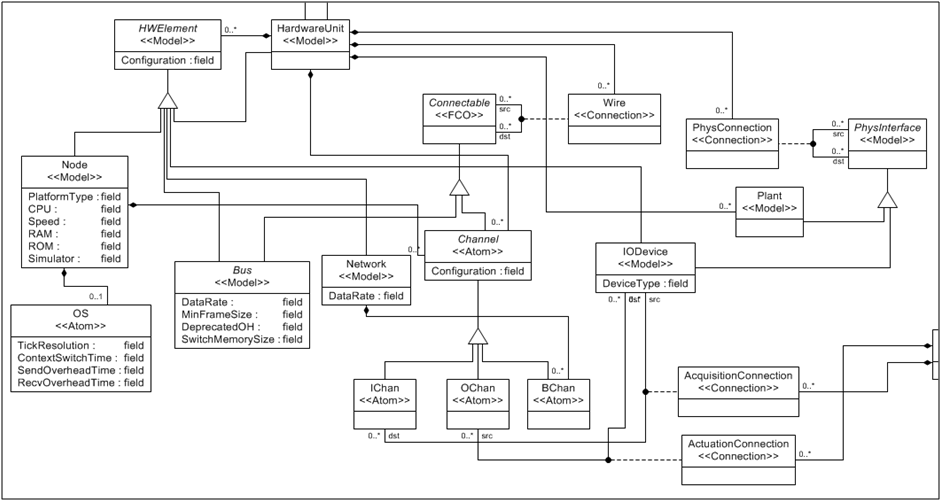
\includegraphics[width=\columnwidth]{figures/platform.png}
	\caption{Platforms. This metamodel describes a simple 
language for modeling the topology of a time-triggered processing 
network.}
	\label{fig:platform}
\end{figure}

The models in the example and the metamodels described below 
were created using the ISIS Generic Modeling Environment 
tool (GME)~\cite{mic:gme}.  GME allows language designers to create 
stereotyped UML-style class diagrams defining metamodels.  
The metamodels are instantiated into a graphical language, 
and metamodel class stereotypes and attributes determine how 
the elements are presented and used by modelers. 

The Model-Integrated Computing (MIC) approach\cite{mic:overview} 
builds up DSMLs by creating specific sublanguages to 
capture concepts and relationships for different facets of the
design domain, and then integrating those sublanguages into 
a common modeling language by precisely specifying the 
structural relationships between those sublanguages.  In a GME
metamodel a sublanguage is called a \emph{paradigm}.  We will
use the terms sublanguage, language, and paradigm interchangeably.
Confusion is resolved by explicitly naming the paradigms involved
in the discussion.

The GME metamodeling syntax may not be entirely familiar 
to the reader, but it is well-documented in Karsai 
et al~\cite{mic:gme}. Class concepts such as inheritance can be 
read analogously to UML.  Class aggregation represents 
containment in the modeling environment, though an aggregate 
element can also be flagged as a port object.  In the modeling 
environment a port object will also be visible at the next 
higher level in the model hierarchy, and available for 
connections.  GME allows the specification of association classes which are visualized as edge connections between objects in models.  For example, the dot 
between the \emph{Connectable} class and the \emph{Wire} association class 
(Fig. \ref{fig:platform}) represents an edge connecting two objects which are subtypes of \emph{Connectable}.  One other useful 
concept from a GME metamodel is the reference, which is a lightweight object that refers to another object somewhere else in the model hierarchy, in much the same way that a pointer references a concrete object in memory.  A reference
object appears in the Metamodel specification associated with
another class, providing a convenient notation for model connections which span the model hierarchy\cite{mic:gme}. This allows the modeler to create a pointer-like object, 
with is visualized with the same interface (port structure) as the associated
class, but which actually refers to the original object.

Another key technology used in the ESMoL tool suite is 
the GReAT model transformation language (and its associated 
code generation tools)\cite{mic:great}.  The ESMoL suite contains a 
pair of platform-independent code generators for Simulink 
and Stateflow models.  The transformations take Simulink 
and Stateflow blocks, and create equivalent models in 
another language (SFC) that corresponds to an abstract 
syntax graph for fragments of C code.  Functional code 
generation proceeds by simply traversing and printing the SFC 
models. Other generators use the UDM C++ modeling API \cite{mic:udm} to 
create code implementing the 
platform-specific code to wrap functions as tasks, define 
communication messages structures, and configure a 
time-triggered virtual machine to execute the generated code.  
These generators as well as generators for platform-resimulation 
models are described elsewhere (see Porter et al \cite{modeling:esmol}, 
Thibodeaux \cite{timed:frodo}, and Hemingway et al
\cite{modeling:truetime} for details).

Platform-based design partitions design frameworks into designer-supplied
components and platform-provided services\cite{modeling:platform}.  
High-confidence systems require services and guarantees 
for correct and efficient execution such as real-time execution, 
data distribution, and fault tolerance.
Platform-based design allows the construction
of complex systems by facilitating reuse over common execution
behaviors. 
The platform also defines a formal model of computation 
(MoC) \cite{sem:taggedsig}, which predicts how the concurrent 
objects of an application interact (i.e. synchronization and 
communication). 
We use an implementation of the time-triggered 
architecture as a platform layer in order to
reduce timing variances in sensing, actuation, and 
distributed data communications \cite{timed:tta}\cite{timed:frodo}.
The central idea of the time-triggered 
architecture is to provide deterministic and fault-tolerant synchronous
execution in order to ensure the consistent behaviors of
distributed replicas of controller components.

\section{The ESMoL Languages}

\begin{figure}
\centering
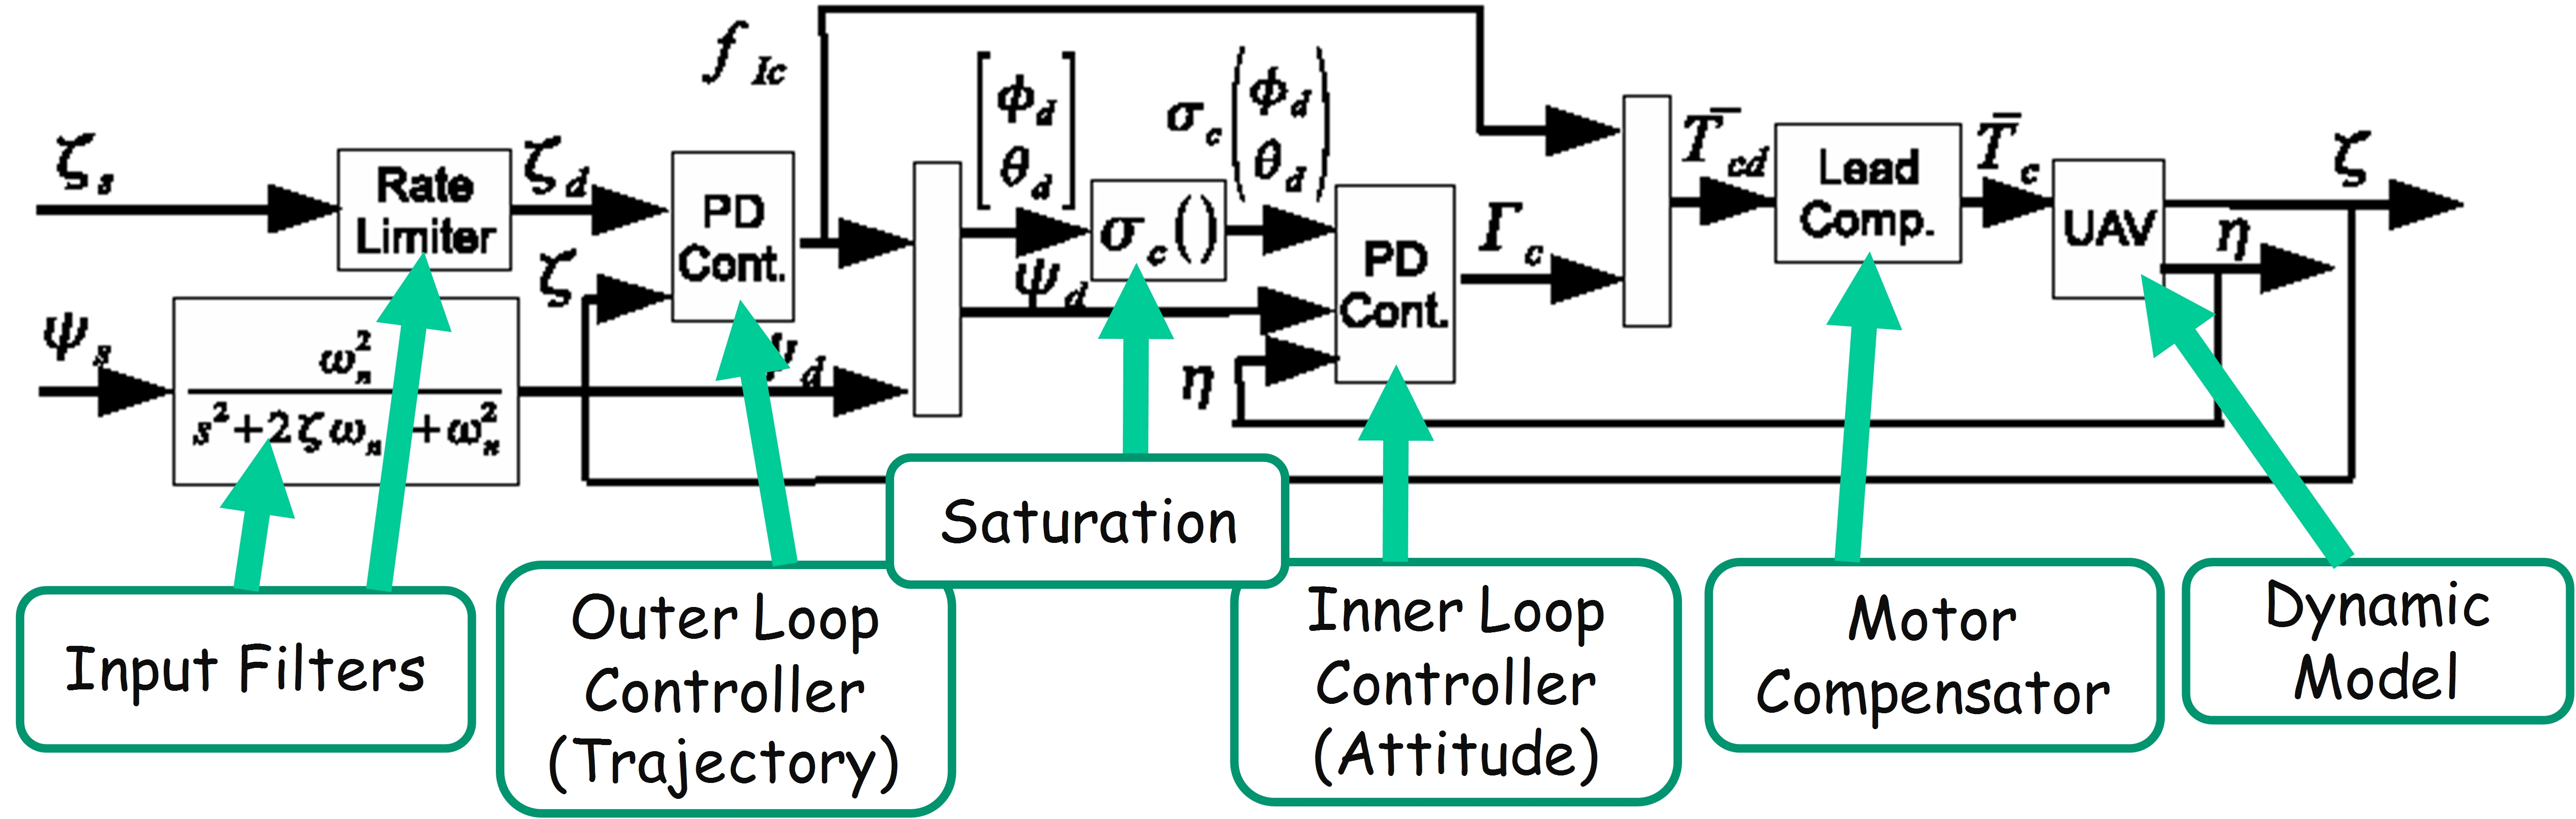
\includegraphics[width=0.8\columnwidth]{figures/quadrotor_arch.png}
    \caption{Basic architecture for the quadrotor control problem.}
    \label{fig:quadrotor}
\end{figure}

To motivate our description of the facets of ESMoL, we focus on an 
actual control design model for the Starmac quadrotor helicopter 
\cite{quad:starmac}\cite{quad:starmacdyn}.  Fig. \ref{fig:quadrotor}
depicts its control architecture, consisting of two nested control loops.
From left to right in the diagram, the \emph{Input Filters} restrict
the input trajectory commands to prevent maneuvers beyond the physically
safe limits of the helicopter.  The \emph{Outer Loop} PD controller 
takes the requested position reference and the position data from the 
sensors, and calculates the attitude required for the quadrotor to
achieve the requested change in position.  \emph{Saturation} is another
limiter to ensure that the commanded attitude actuation is realizable.
The \emph{Inner Loop} PD controller takes the attitude command from
the \emph{Outer Loop} and measured attitude data, and calculates 
the motor thrusts required to achieve the commanded attitude.
\emph{Motor Compensator} filters the thrust commands to account for 
response delays in the motors which drive the rotors.  Finally, the 
\emph{Dynamic Model} describes the physical behavior of the helicopter,
including the imprecision introduced by the sensors which measure
position and attitude.
The ESMoL model examples given below come from the design model for
the quadrotor, except where noted.

\subsubsection*{Requirements Analysis (RA)}

Formal requirements modeling offers great promise, 
but in ESMoL requirements modeling is still in conceptual stages.  
Informally, we require stability of the software-implemented 
closed-loop control system 
over the full range of possible inputs, and satisfaction of the
calculated timing constraints (task release times and deadlines).

\subsubsection*{Functional Design (FD)}

In ESMoL, functional specifications for components 
can appear in the form of Simulink/Stateflow models or 
as existing C code snippets.  ESMoL does not support 
the full semantics of Simulink. In ESMoL the execution 
of Simulink data flow blocks is restricted to periodic 
discrete time, consistent with the underlying 
time-triggered platform.  This also restricts the type 
and configuration of blocks that may be used in a 
design.  Continuous integrator blocks and sample time 
settings do not have meaning in ESMoL.  C code snippets 
are allowed in ESMoL as well.  C code definitions are 
limited to synchronous, bounded response time function 
calls which will execute in a periodic task with a fixed
amount of memory.

An automated importer constructs an ESMoL model from a
Simulink control design model.  The new model is a structural
replica of the original Simulink model, only endowed with a 
richer software design environment and tool-provided APIs for 
navigating and manipulating the model structure in code.  
The Simulink and Stateflow sublanguages of our modeling 
environment are described elsewhere\cite{mic:ecsldp}.  
The ESMoL language evolved from another DSML known as 
ECSL-DP.  They share many
concepts, but ESMoL departs from many of the modeling
structures previously described by Neema in order to increase
the flexibility and generality of the language.

\subsubsection*{Component Design (CD)}

\begin{figure}
\centering
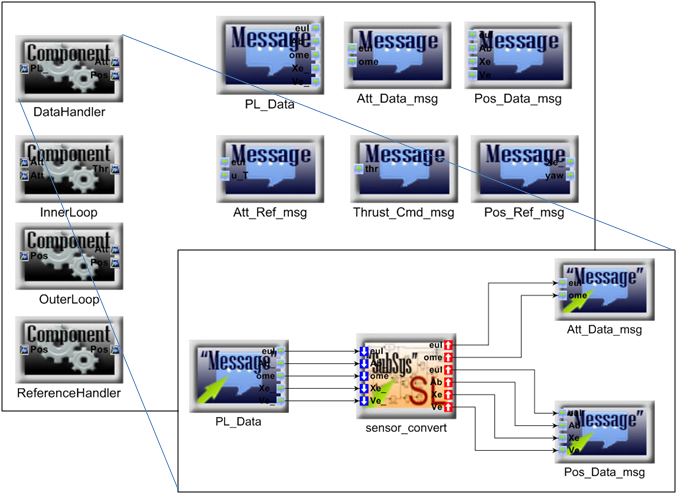
\includegraphics[width=0.85\columnwidth]{figures/quadrotor_types.png}
    \caption{Quadrotor component types model from the \emph{SysTypes} paradigm.}
    \label{fig:qr_types}
\end{figure}

In the component design phase (CD) we specify 
software interfaces for the functions which will run in the 
distributed controller network.  
A component type has a
unique name (i.e. \emph{InnerLoop}), and information to find or generate its
implementation in C (in this case, the file name and model path 
to the Simulink subsystem ``QuadRotor/STARMAC/InnerLoop'').
A component specification 
contains a reference to a Simulink subsystem,
as well as references to message structure objects. 
The message structure objects will represent message
types, and each reference from a component definition 
represents an interface through which that message
is sent or received.  Internally, the direction of 
the connection from the message reference to the ports
on the Simulink object determine whether the port 
sends or receives.  We do not allow multi-directional
message transfers on the same interface.  When the 
component is instantiated in the design model
(e.g., in the logical architecture diagram described 
below) the message references specified here will 
appear as ports on blocks representing the instance.  
Connections to and from those ports represent the transfer of 
an instance of that data message into or out of the component instance.

Fig. \ref{fig:qr_types} shows an example of a model from the 
component interface definition language.  Message fields 
and their sizes are specified here, as well as component 
implementations and interfaces.  These specifications define 
software component types in an ESMoL model, which are instantiated 
and assigned to hardware in the architecture and deployment models,
respectively.  The quadrotor 
model has four different component types (each instantiated once) 
and six message types (instantiated as the ports objects appearing 
on the component instances later in the design).  The breakout inset in 
the figure shows the internals of the \emph{DataHandler} component 
specification.  The \emph{sensor\_convert} subsystem block 
in the center is a reference to a Simulink block specifying the data
conversions that transform raw sensor data into scaled, formatted
data for use by the controller blocks.

The blocks on the outer edges of the figure (Fig. \ref{fig:qr_types}) 
are references to messages 
defined at the top level of the system types model. 
On the left is the raw data message from the sensors.  On the right are
the attitude data message (for local consumption by the inner loop), and 
the position data message (sent remotely to the outer loop). 
The three message reference blocks in the inset appear as ports on the 
\emph{DataHandler} block (top left in the figure).  Inside the 
component type definition, ports on the message objects 
correspond to C structure fields. The field types are
inferred from the data types imported from the connected Simulink
signal port objects. The 
connections between the message ports and the Simulink 
reference block ports describe the direction and details 
of data flow between the implemented message structures 
and the specified functional block.

\begin{figure}
	\centering
	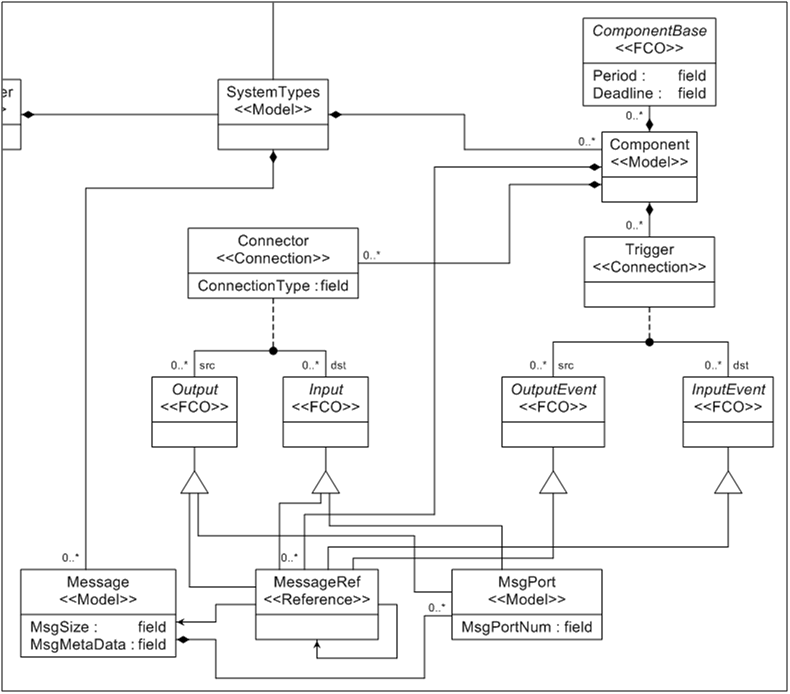
\includegraphics[width=0.85\columnwidth]{figures/arch_lang.png}
	\caption{SystemTypes Metamodel.} 
	\label{fig:arch}
\end{figure}

Fig. \ref{fig:arch} portrays the \emph{SystemTypes} sublanguage, 
which encodes these structures and relations.  
Components of different types (here Simulink block references 
or C code blocks) specify the component functions.  Message 
references (\emph{MessageRef} objects) define interfaces 
on the components, and ports on message objects (\emph{MsgPort} objects)
represent message data fields as in the \emph{DataHandler} example.  
The \emph{Input} and \emph{Output} 
port classes are typed according to the implementation 
class to which they belong (i.e., either Simulink signal 
ports or C function arguments). The connections between the 
block reference and the \emph{MsgPort} objects describe the details 
required to marshal and demarshal the data fields in the messages 
for use by the specified function.  
Synchronous, periodic, discrete-time Simulink blocks and bounded-time
synchronous C function calls are compatible at this modeling 
stage, because their model 
elements both represent the code that will finally implement the 
functions.  These units are modeled as blocks with ports, where the ports 
represent parameters passed into and out of C function calls.
The \emph{Trigger} and \emph{Event} types are not discussed here,
as they relate to future work in the ESMoL tool suite.

\subsubsection*{Hardware Architecture (HwA)}

\begin{figure}
  \centering
  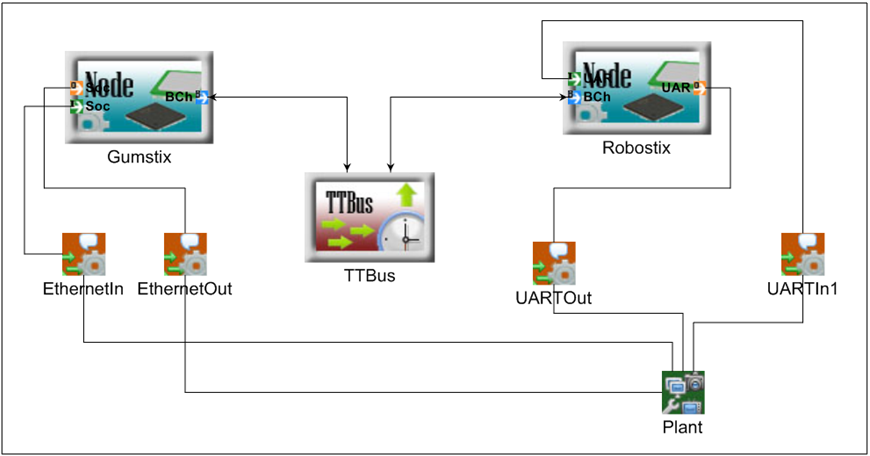
\includegraphics[width=0.8\columnwidth]{figures/quadrotor_hardware.png}
  \caption{Overall hardware layout for the quadrotor example.}
  \label{fig:qr_hardware}
\end{figure}

Fig. \ref{fig:qr_hardware} illustrates the example
platform model.  The quadrotor architecture
is deployed to a small embedded processor assembly 
manufactured by Gumstix, Inc.
The outer loop position control is handled by an Intel
PXA ARM processor (the Gumstix 
board), and attitude control and vehicle I/O are 
handled by an Atmel Atmega128 AVR processor (the 
Robostix board).  The I/O occurs over serial 
connections to the sensors and motor actuators.  
The serial devices reside within the processor, and are 
modeled in the diagram as objects connecting the 
input and output ports on the processor to the object 
representing the plant dynamics.  The two processors 
communicate via a synchronous $I^2C$ bus which runs
a software emulated time-triggered protocol.

A simple platform definition language (Fig. \ref{fig:platform}) 
contains relationships and attributes describing time-triggered 
networks.  The models contain network topology and parameters to describe 
behavioral quantities like data rates and bus transfer setup times.
Platforms are defined 
hierarchically as hardware units with ports for 
interconnections. Primitive components include 
processing nodes and communication buses.  Behavioral 
semantics for these networks come from the underlying 
time-triggered architecture.  The time-triggered 
platform provides services such as deterministic 
execution of replicated components and timed 
message-passing.  Model attributes for hardware also 
capture timing resolution, overhead parameters for 
data transfers, and task context switching times.

\subsubsection*{Architecture Language}

Logical architecture, deployment, and timing/execution
models represent different design aspects for the same set 
of component instances.  GME allows us to define the 
language in such a way that these three model aspects are 
simply different views of the same set of model elements.
Together, the information in the three aspects define a model
which is complete with respect to scheduling analysis,
platform-specific simulation, and code generation.

System design models defined in the architecture language do not 
necessarily represent complete designs.  For simple designs (such as 
the quadrotor example) a single architecture model can capture all of 
the details of the software model.  More complex designs require an
additional layer of organization which is not described here.  It
suffices to say that designs represented in the ESMoL Architecture 
language can be considered as fragments which can be assembled into
more complex structures.  This is an active area of research for
our ESMoL modeling efforts, as the higher-level architecture models
should also account for fault modeling, evaluation, and performance issues.

\begin{itemize}

\item \textbf{Logical Software Architecture (SwA) Aspect} 
Fig. \ref{fig:qr_log_arch} portrays an ESMoL model example 
specifying logical data dependencies between 
quadrotor software component instances, 
independent of their distribution over different
processors.  The software architecture model 
describes the logical dataflow dependency relationships between component 
instances.  
Semantics for SwA Connections are those of task-local 
synchronous function invocations (with shared memory messaging)
or message transfers between remote tasks using 
time-triggered communication.  In this model the interpretations
for the dependency links have not been specified.  Those details
appear in the deployment model.

For the quadrotor, the \emph{RefHandler} and \emph{DataHandler}
components receive and process data from the sensors.  They pass
their formatted data to the respective control blocks.  The 
\emph{OuterLoop} calculates an attitude reference to achieve the
requested position.  The \emph{InnerLoop} issues thrust commands
to achieve the requested attitude.

In a design model, creation of a (GME) reference object to one of the 
component types corresponds to instantiation.
Fig. \ref{fig:qr_tmr} illustrates this idea.  Using 
the same controller components along with a few new
components to implement voting logic, we have specified 
the logical architecture for a triply-redundant
version of the quadrotor model.  Each ESMoL component
type is used multiple times in a single design, expanding 
the model structure far beyond the size and scope of the
original Simulink design.  This 
particular model diagram is only shown to 
illustrate the instantiation mechanism.

\begin{figure}
\centering
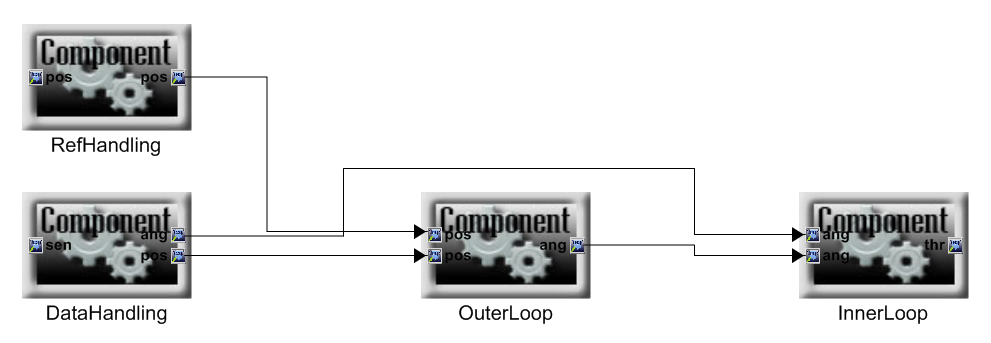
\includegraphics[width=0.8\columnwidth]{figures/quadrotor_log_arch.png}
    \caption{Quadrotor architecture model, Logical Architecture aspect.}
    \label{fig:qr_log_arch}
\end{figure}

\begin{figure}
\centering
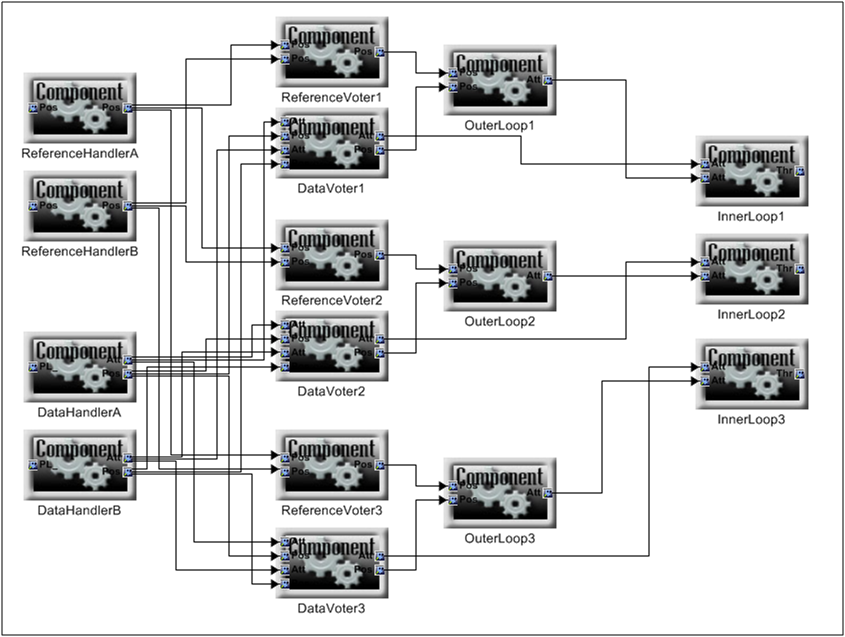
\includegraphics[width=0.6\columnwidth]{figures/qr_tmr.png}
    \caption{Triply-redundant quadrotor logical architecture.  This is 
not part of the actual quadrotor model, and is only given for illustration.}
    \label{fig:qr_tmr}
\end{figure}

\begin{figure}
\centering
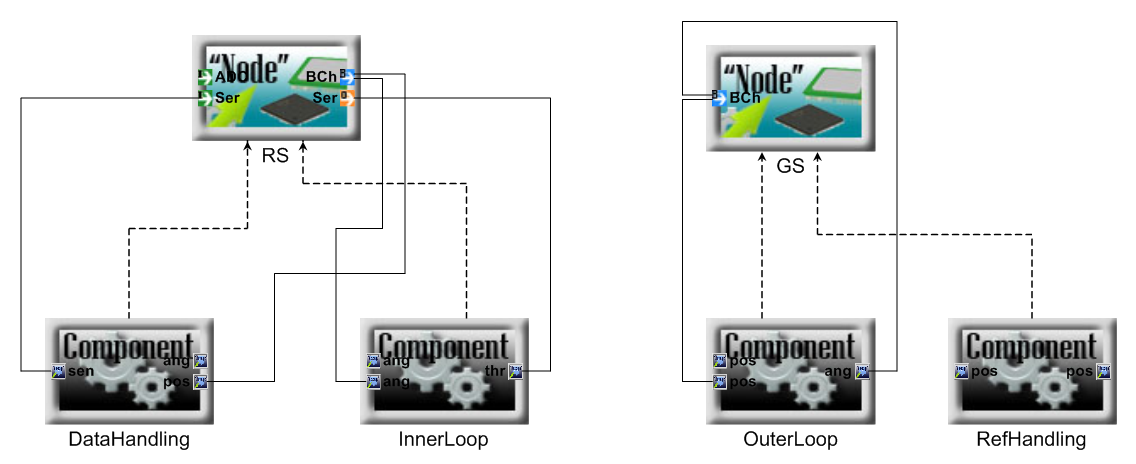
\includegraphics[width=0.8\columnwidth]{figures/quadrotor_hw_mapping.png}
    \caption{Quadrotor architecture model, Deployment aspect.}
    \label{fig:qr_hw_mapping}
\end{figure}

\item \textbf{Deployment Models (SY, DPL)}
Fig. \ref{fig:qr_hw_mapping} displays the deployment model -- 
the mapping of software components to processing nodes, and data 
messages to communication ports.  Two of the four components are 
mapped to each of the two processors.  For the quadrotor, the
\emph{RefHandler} and \emph{OuterLoop} tasks run on the Gumstix
processor.  The \emph{InnerLoop} and \emph{DataHandler} tasks 
run on the Robostix processor.  \emph{RefHandler} receives position
commands from a socket connection.  \emph{DataHandler} receives 
sensor data from a UART channel (a processor port in the model
diagram).  Position and attitude data are exchanged over the
time-triggered bus, so the corresponding message ports are 
connected to bus channel objects on their respective processors.
\emph{InnerLoop} sends thrust commands through a UART channel,
hence the connection to the appropriate processor port.

In the figure the dashed connection from 
a component to a node reference represents an assignment of 
that component to run as a task on the node.  The port 
connections represent the hardware channel through which 
that particular message will travel.  Remote message dependencies 
are assigned to bus channels on the node.  Local data 
dependencies are not specified here, as they are represented 
in the logical architecture.  \emph{IChan} and \emph{OChan} port 
objects on a node can also be connected to message objects on a component.  
These connections represent the flow of data from the physical 
environment through sensors (\emph{IChan} objects) or the flow of 
data back to the environment through actuators
(\emph{OChan} objects).  Model interpreters use deployment models to 
generate platform-specific task wrapping and communication 
code as well as scheduling problem specifications.

\begin{figure}
	\centering
	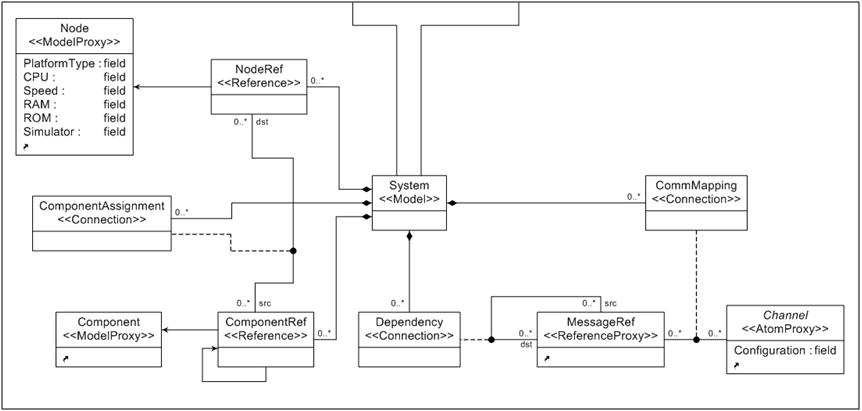
\includegraphics[width=0.85\columnwidth]{figures/depnew.png}
	\caption{Details from the deployment sublanguage.}
	\label{fig:depnew}
\end{figure}

The metamodel in Fig. \ref{fig:depnew} illustrates the 
classes and relationships for both the logical
architecture connections and the deployment mapping.  
GME metamodels have a separate visualization 
aspect that allows us to define aspects in ESMoL and 
indicate which classes and connections should be
visible in each aspect.  \emph{ComponentRef} objects are 
software component instances, and are visible in both aspects.
In the logical architecture aspect, \emph{Dependency} connectors 
define message transfers between component instance ports.  
The ports represent interfaces for each component instance.  
For the deployment aspect we add \emph{NodeRef} objects (node references) 
and connectors (\emph{ComponentAssignment} and \emph{CommMapping}) to identify
the mapping of tasks and messages to the platform model.

The deployment aspect captures the assignment of component 
instances as periodic tasks running on a particular processor.  
In ESMoL a task executes on a processing node at a single 
periodic rate.  All components within the task execute 
synchronously.  Data sent between tasks take the form of 
messages in the model.  For data movement, the runtime
provides logical execution 
time semantics found in time-triggered languages such as 
Giotto~\cite{timed:giotto} -- message transfers are scheduled 
after the deadline of a sending task, but before the release 
of the receiving tasks.  Tasks never block, but execute with 
whatever data is available for each period.

\begin{figure}
\centering
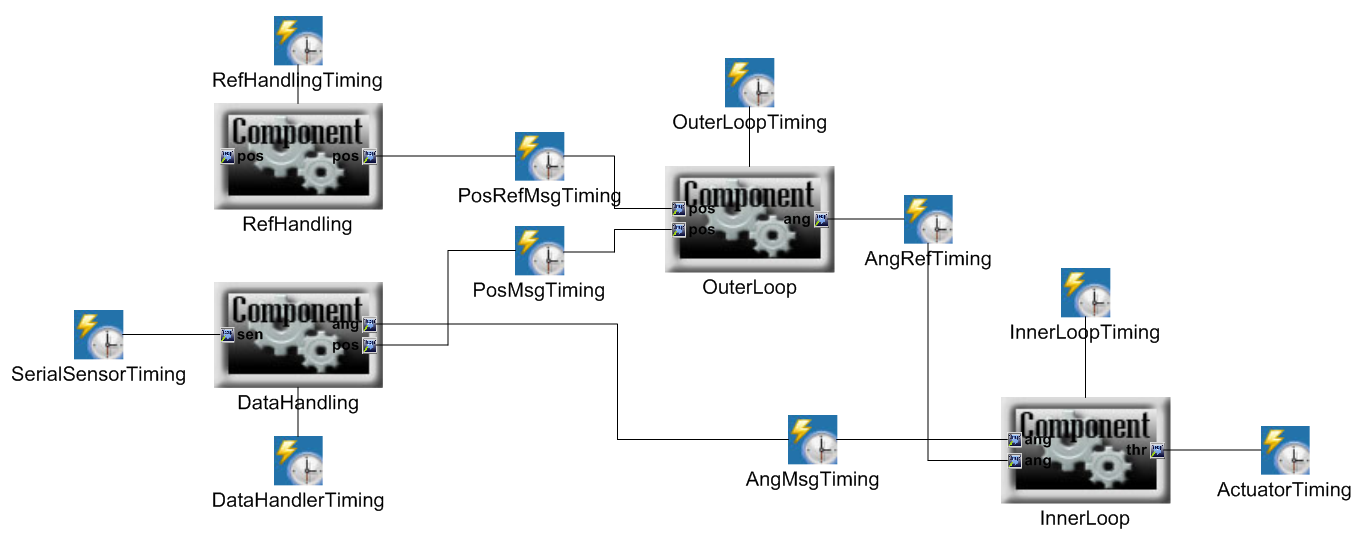
\includegraphics[width=0.9\columnwidth]{figures/quadrotor_timing.png}
   \caption{Quadrotor architecture model, Timing aspect.}
   \label{fig:qr_timing}
\end{figure}

\item \textbf{Timing Models}
Fig. \ref{fig:qr_timing} shows the quadrotor timing and execution model,
where the designer attaches
timing parameter blocks (of type \emph{TTExecInfo}) to components 
and messages.  \emph{TTExecInfo} block configuration 
parameters include execution period and 
worst-case execution time.  In the quadrotor model all 
task and message transfers are timed.  The quadrotor data
network runs at a rate of $20 ms$.  Particular timings for
tasks and data transfers will be discussed below in the
evaluation discussion.

\begin{figure}
	\centering
	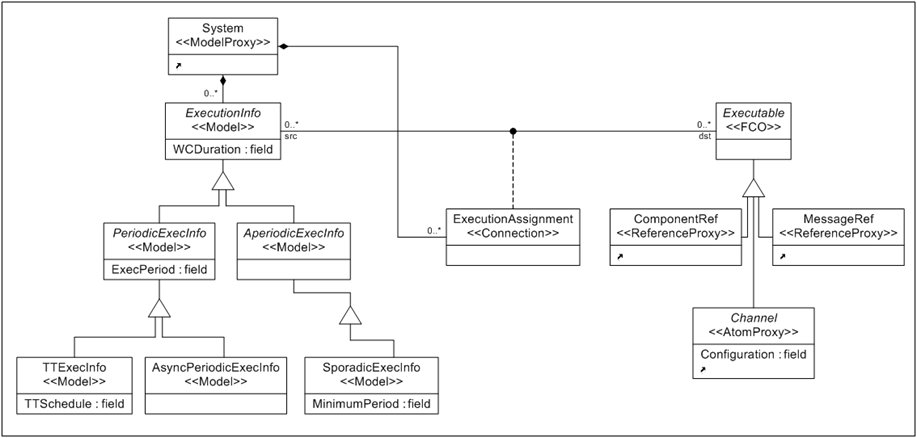
\includegraphics[width=0.85\columnwidth]{figures/timing.png}
	\caption{Details from timing sublanguage.}
	\label{fig:timing_lang}
\end{figure}

The timing sublanguage (Fig. \ref{fig:timing_lang}) allows 
the designer to specify component execution
constraints.  Individual components can be annotated with 
timing objects that indicate whether they should be executed 
strictly (i.e., via statically scheduled time-triggered means), 
or as periodic real-time or sporadic tasks. 
Messages are similarly annotated.  
The annotation objects contain parameters such as period and 
worst-case execution time that must be given by the designer.  
Automated scheduling analysis fills in the schedule fields.

The execution model also indicates which components and messages 
will be scheduled independently, and which will be
grouped into a single task or message object. 
The time order of the message writer and readers are enforced 
by the static schedule. The locality of a message transfer is
specified in the logical architecture and deployment aspects. 
In the case of processor-local data transfers, transfer time is 
neglected -- reads and writes occur in locally shared memory. 
After a static schedule has been calculated, task and message 
release times are also stored in the timing objects.

Behavior of the deployed 
software components depends on the execution times of 
the functions on the platform, the calculated schedule, 
and coordination between distributed tasks. The 
calculated static execution schedule can be used to simulate the 
control design with additional delays to assess the impact 
of the platform on performance.

\end{itemize}

\section{Integrating Tools with ESMoL}
\label{section:twostage}

Figure \ref{fig:designflow} depicts a design flow 
that includes a user-facing modeling language 
for design and an abstract intermediate language 
for supporting interpreter development and
maintenance.  A completed ESMoL model is 
transformed (via the Stage 1 
transformation, Step 6 in the figure) into a model in the ESMoL\_Abstract 
language, where all implied relationships and structural 
model inferences have been resolved.  Model interpreters 
for calculating time-triggered schedules, creating 
platform-specific simulations, and generating deployable 
code are integrated using the Stage 2 transformation.


Rather than designing a user-friendly graphical modeling 
language and directly attaching translators
to analysis tools, we created a simpler abstract 
intermediate language whose elements are similar to 
those of the user language. The first model transformation 
flattens the user model into the abstract intermediate form,
translating parameters and resolving special cases as needed. 
Generators for code and analysis are attached to the abstract 
modeling layer, so the simpler second-stage transformations 
are easier to maintain, and are isolated from changes to 
the user language.

In the model integrated computing approach, domain specific 
modeling languages represent different aspects of the design, 
with the aim  of consistently integrating different concepts 
and details for those design aspects and integrated analysis tools.
Our tools enforce a single view of structural inference in the 
design model. We will cover some of the transformation details 
to illustrate this concept.
This approach can be considered as an implementation of the tool 
integration ideas in \cite{modeling:hybrid_abs}, but with variations 
of the details included in the design language.  

\subsection{Stage 1 Transformation}
\label{sect:stage1}

\begin{figure}
\centering
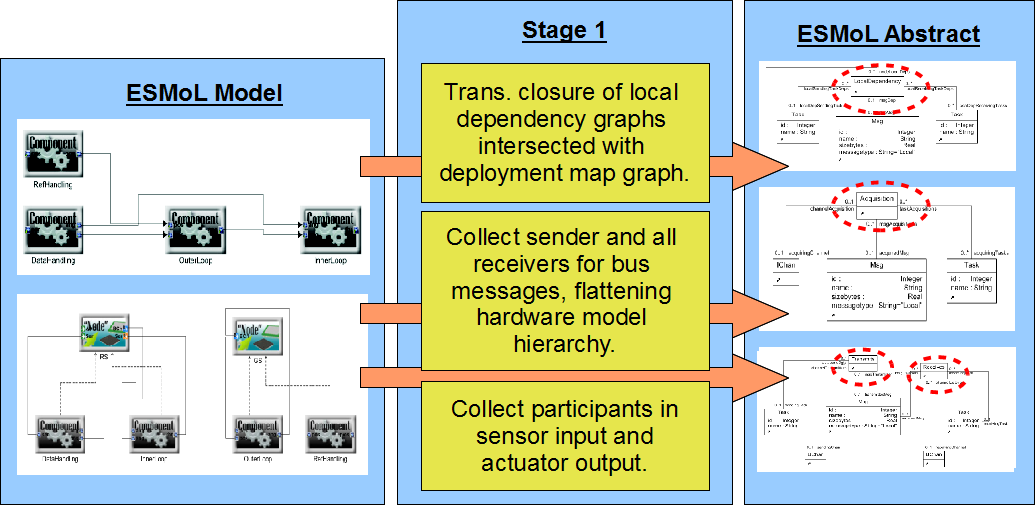
\includegraphics[width=0.95\columnwidth]{figures/stage1.png}
   \caption{Stage 1 Transformation.}
   \label{fig:stage1}
\end{figure}

\begin{table*}
\centering

\begin{tabular}[width=0.5\columnwidth]{ | l | l | }
 \hline
 \textbf{Specified ESMoL Relation Sets} & \textbf{ESMoL\_Abstract Relation} \\
 \hline \hline
                                                                        & \\
 $CA_{id_N} = \{ (obj_{Node}, obj_{CompInst} ) \, |$                    & \\
 \hspace{1.7cm} $ id(obj_{Node}) = id_N \} $                            & \\
                                                                        & \\
 $AC_{id_{Ch}} = \{ (obj_{IChan}, obj_{MsgInst} ) \, |$                 & 
$ Acq = \{(obj_{MsgInst}, obj_{CompInst}, $  \\
 \hspace{1.6cm} $id(obj_{IChan}) = id_{Ch} \} $                         & 
\hspace{1.3cm} $obj_{N}, obj_{Ch}) \, |$ \\
                                                                        &  
\hspace{0.8cm} $(obj_{N}, obj_{CompInst}) \in CA_{id_N}$ \\
 $NC_{id_N} = \{ (obj_{Node}, obj_{IChan}) \, | $                       & 
\hspace{0.5cm} $ \wedge \, (obj_{Ch}, obj_{MsgInst}) \in AC_{id_{Ch}}$ \\
 \hspace{1.35cm} $id(obj_{Node}) = id_N $                                &
\hspace{0.5cm} $ \wedge \, (obj_{N}, obj_{IChan}) \in NC_{id_N}$ \\ 
 \hspace{1cm} $ \wedge \, parent(obj_{IChan} ) = obj_{Node} \}$       &
\hspace{0.5cm} $ \wedge \, (obj_{CompInst}, obj_{MsgInst}) \in CC $ \\
                                                                        & \\
 $CC = \{ (obj_{CompInst}, obj_{MsgInst} ) \, | $                       & \\
 \hspace{0.7cm} $parent(obj_{MsgInst} ) = obj_{CompInst} \}$            & \\ 
                                                                        & \\
 \hline
\end{tabular}
	\caption{Acquisition relation transformation details.}
	\label{tab:acquisition}
\end{table*}

\begin{figure}
\centering
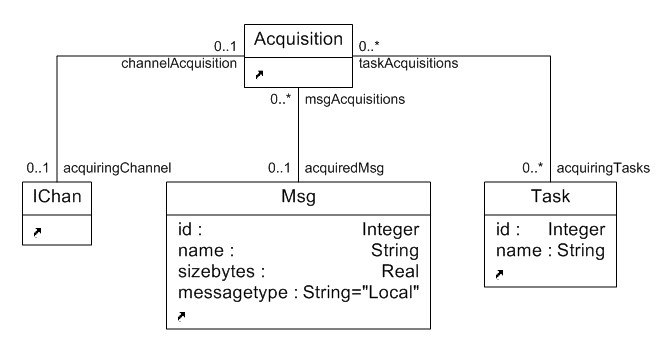
\includegraphics[width=0.8\columnwidth]{figures/acquisition.png}
    \caption{Acquisition relation in ESMoL Abstract, representing the
timed flow of data arriving from the environment.}
    \label{fig:acq_meta}
\end{figure}

Stage 1 translates ESMoL models into an abstract intermediate language that
contains explicit relation objects that represent relationships implied by
structures in ESMoL (Fig. \ref{fig:stage1}). This translation is similar to the way a compiler translates concrete syntax first 
to an abstract syntax tree, and then to intermediate semantic representations suitable for optimization.  
Stage 1 was implemented using the UDM model navigation
API, and written in C++.  The ESMoL\_Abstract target model is the source for
the transformations implemented in Stage 2.

Each analysis translation works from a single view of the design model, 
simplifying the implementations of tool-specific translations.  
As an example, consider the model
shown in Fig. \ref{fig:qr_log_arch}.   Component
\emph{DataHandler} sends data messages to the other two components, as denoted by the
dependency arrows.  The deployment
view (Fig. \ref{fig:qr_hw_mapping}) shows that each component executes on a
different processor.  Locally, the port object on each component (in both
diagrams) represents the component's view of the data message sent over
the wire. The solid connections in the deployment diagram indicate which device
on the processing node will be used to transfer the data.  Specified messages
will participate in processor-local synchronous data flows, or time-triggered
exchanges over the network.  All of these connections and entities are related
to a single semantic message object, which is related to other elements in
different parts of the user model (see the FormattedData message in Fig.
\ref{fig:msg_sched}).  The execution aspect contains timing
information objects, which provide information for fully specifying
the various data transfers.

The first stage transformation checks constraints to ensure that each object 
is used correctly throughout the design, ensuring well-formedness.  
The Stage 1 transformation then reduces this complex set of relations
to a single message object with relations to the other objects that use it. 
Timing parameters from the platform model are used to calculate a behavioral
model for messages and components, including component start times, message 
transfer times, and the duration of each message on the bus.

We describe here some of the transformations of user-facing 
ESMoL language objects and
relations to a more compact set of relations that simplify generation of design
artifacts from the model.  The most direct example of such a semantic assumption
is the single-message abstraction.  Data transfers between the functional code
and the message fields must be compatible. We enforce compatibility 
both by constraint
checking, and by the use of a single ESMoL\_Abstract message instance 
object for all
participants in the data interchange.  The \emph{Signal} object in the
abstract graph represents the transfer of a single datum to or from the message.
For simplicity and clarity we will not show the \emph{Signal} objects in the diagrams, as they are numerous.

The transformations described here capture different forms of the
single-message transformation.  This is not a complete description of the
entire first stage transformation, but provides a representative subset for
illustration.

In the formal descriptions below, $Obj_{Type}$ (capitalized) is the set of objects of type $Type$, and
$obj_{Type}$ (lowercase) is an instance from that set.  We also
use two functions $id: Obj_{Type} \rightarrow \mathbf{Z}^{+}$ for a unique
identifier of an object, and $parent: Obj_{Type1} \rightarrow Obj_{Type2}$ to
find the parent (defined by a containment relation in the model of an object).
The parent relation is unique.

\textbf{Acquisition: From the Environment to Data}

In ESMoL\_Abstract \emph{Acquisition} objects relate all of the different model entities (and
therefore, their design parameters) that participate in the collection of data
from an input device such as an analog to digital converter or serial link. 
The Stage1 transformation enforces certain cardinality constraints to ensure
the validity of this transformation -- for example, each message instance is 
related to exactly one sender and possibly multiple receivers.  A message 
relationship can be implied by different types of connections in ESMoL, so 
Stage1 must determine that only one such relationship exists.

The ESMoL relations shown in Table \ref{tab:acquisition} are 
described as follows:

\begin{itemize}
 \item $CA$ {\bf ComponentAssignment}: (the dashed connection shown in 
Fig. \ref{fig:qr_hw_mapping}) assigns a task to run on a particular 
processor ($id_N$).
 \item $AC$ {\bf AcquisitionConnection}: (the directed connection from 
processor object ports to component message ports) assigns a hardware input peripheral
data channel (modeled as an object of type $IChan$) to a data-compatible 
message structure in the component.
 \item $NC$: Containment relationship of the channel object (port) in the Node object.
 \item $CC$: Containment of the message instance object (port) in the component instance object.
\end{itemize}

The metalanguage for ESMoL\_Abstract captures the structural
semantic reductions shown in Table \ref{tab:acquisition} in a compact form (see Fig. \ref{fig:acq_meta}), so that all of the consumers of the input data get the same consistent structural view of the model. This transformation takes the ESMoL objects described in the left column of the table and produces a single relation for each
collection representing an ESMoL\_Abstract data acquisition specification. The modeling tools provide a programming interface for traversing, reading, and editing the models.
The collected relations are also more efficiently processed by 
synthesis interpreters, as they avoid extra traversals to gather the 
objects.  

\textbf{Actuation: From Data to the Environment}

\begin{table*}
\centering

\begin{tabular}[width=0.5\columnwidth]{ | l | l | }
 \hline
 \textbf{Specified ESMoL Relation Sets} & \textbf{ESMoL\_Abstract Relation} \\
 \hline \hline
                                                                        & \\
 $CA_{id_N} = \{ (obj_{Node}, obj_{CompInst} ) \, |$                    & \\
 \hspace{1.7cm} $ id(obj_{Node}) = id_N \} $                            & \\
                                                                        & \\
 $AC_{id_{Ch}} = \{ (obj_{OChan}, obj_{MsgInst} ) \, |$                 & 
$ Act = \{(obj_{MsgInst}, obj_{CompInst}, $  \\
 \hspace{1.6cm} $id(obj_{OChan}) = id_{Ch} \} $                         & 
\hspace{1.3cm} $obj_{N}, obj_{Ch}) \, |$ \\
                                                                        &  
\hspace{0.8cm} $(obj_{N}, obj_{CompInst}) \in CA_{id_N}$ \\
 $NC_{id_N} = \{ (obj_{Node}, obj_{OChan}) \, | $                       & 
\hspace{0.5cm} $ \wedge \, (obj_{Ch}, obj_{MsgInst}) \in AC_{id_{Ch}}$ \\
 \hspace{1.35cm} $id(obj_{Node}) = id_N $                               &
\hspace{0.5cm} $ \wedge \, (obj_{N}, obj_{OChan}) \in NC_{id_N}$ \\ 
 \hspace{1cm} $ \wedge \, parent(obj_{OChan} ) = obj_{Node} \}$         &
\hspace{0.5cm} $ \wedge \, (obj_{CompInst}, obj_{MsgInst}) \in CC $ \\
                                                                        & \\
 $CC = \{ (obj_{CompInst}, obj_{MsgInst} ) \, | $                       & \\
 \hspace{0.7cm} $parent(obj_{MsgInst} ) = obj_{CompInst} \}$            & \\ 
                                                                        & \\
 \hline
\end{tabular}
	\caption{Actuation relation transformation details.}
	\label{tab:actuation}
\end{table*}

\begin{figure}
\centering
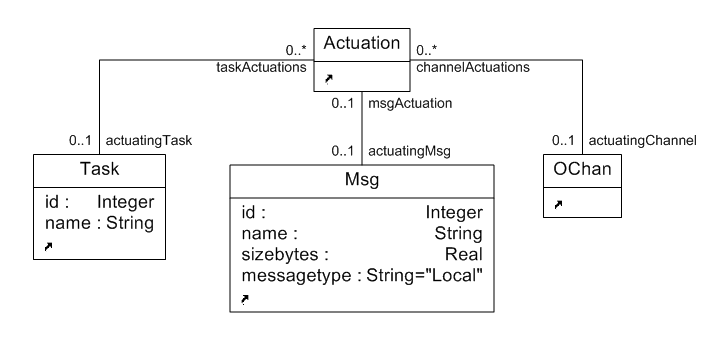
\includegraphics[width=0.8\columnwidth]{figures/actuation.png}
    \caption{Actuation relation in ESMoL Abstract, representing the
timed flow of data back into the environment.}
    \label{fig:act_meta}
\end{figure}

The transformation to an Actuation object is nearly identical to that of the 
Acquisition transformation, but the data direction, cardinalities, and types 
involved are different.  The chief difference is that actuation objects can
only have one associated task, where acquisition data may be broadcast
to multiple tasks.  Table \ref{tab:actuation} gives the details of the
transformation from relations in ESMoL to the actuation relation in 
ESMoL\_Abstract.  Fig. \ref{fig:act_meta} shows the structure of the 
resulting classes in ESMoL\_Abstract.

%\subsection{Local Dependencies: Data Movement within Nodes}
\textbf{Local Dependencies: Data Movement within Nodes}
Local dependencies represent not only direct data dependencies between nodes on
a particular processor, but also implied dependencies through remote data
transfer chains starting and ending on the same processor.   This is modeled as
the set $LD_{TC}$ of all pairs in the transitive closure of dependencies
starting with the message instance $obj_{MsgInst1}$. The collected set of local
dependencies ( $Locals$ ) intersects this set with those message instances
contained in components on the current processing node (i.e. from the set $CA_{id_N}$).
Table \ref{tab:localdeps} gives the transformation details.


\begin{table*}
\centering

\begin{tabular}[width=0.5\columnwidth]{ | l | l | }
 \hline
 \textbf{Specified ESMoL Relation Sets} & \textbf{ESMoL\_Abstract Relation} \\
 \hline \hline
                                                                        & \\
 $CA_{id_N} = \{ (obj_{Node}, obj_{CompInst} ) \, |$                    & \\
 \hspace{1.7cm} $ id(obj_{Node}) = id_N \} $                            & \\
                                                                        & 
$ Locals = \{(obj_{MsgInst1}, obj_{CompInst1}, $  \\
 $LD_{id_1} = \{ (obj_{MsgInst1}, obj_{MsgInst} ) \, |$             & 
\hspace{0.7cm} $obj_{MsgInst2}, obj_{CompInst2}, obj_{N}) \, |$ \\
 \hspace{1.9cm} $id(obj_{MsgInst1}) = id_1 \} $                & 
\hspace{0.5cm} $(obj_{N}, obj_{CompInst1}) \in CA_{id_N}$ \\
                                                                        &  
\hspace{0.2cm} $\wedge \, (obj_{N}, obj_{CompInst2}) \in CA_{id_N}$ \\
 $LD_{TC} = \{ (obj_{MsgInstj}, obj_{MsgInstj+1}) |  $ & 
\hspace{0.2cm} $ \wedge \, (obj_{MsgInst1}, obj_{MsgInst2}) \in LD_{TC}$
\\
 \hspace{0.3cm} $ in \, the \, sequence  $ &
\hspace{0.15cm} $ \wedge \, (obj_{CompInst}, obj_{MsgInst}) \in CC $ \\
 \hspace{0.4cm} $  ( (obj_{MsgInst1}, obj_{MsgInst2}) \in LD_{id_1}, $ &
\\
 \hspace{0.4cm} $ (obj_{MsgInst2}, obj_{MsgInst3}) \in LD_{id_2}, $ & \\
 \hspace{0.7cm} \dots & \\
 \hspace{0.4cm} $ (obj_{MsgInstj}, obj_{MsgInstj+1}) \in LD_{id_j} ) \} $
& \\
 & \\
 $CC = \{ (obj_{CompInst}, obj_{MsgInst} ) \, | $  & \\
 \hspace{0.3cm} $parent(obj_{MsgInst} ) = obj_{CompInst} \}$ & \\
 & \\
 \hline
\end{tabular}
	\caption{Local (processor-local) data dependency relation.}
	\label{tab:localdeps}
\end{table*}

\begin{figure}
\centering
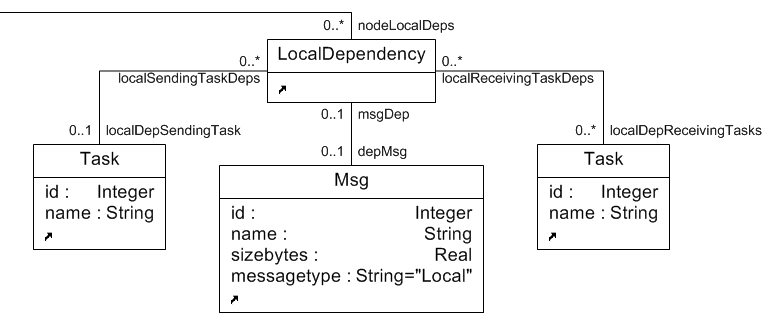
\includegraphics[width=0.8\columnwidth]{figures/localdeps.png}
    \caption{Local dependency relation in ESMoL Abstract, representing data
transfers between components on the same processing node.}
    \label{fig:localdep_meta}
\end{figure}

\begin{table*}
\centering

\begin{tabular}[width=0.5\columnwidth]{ | l | l | }
 \hline
 \textbf{Specified ESMoL Relation Sets} & \textbf{ESMoL\_Abstract Relation} \\
 \hline \hline
                                                                        & \\
 $CA_{id_N} = \{ (obj_{Node}, obj_{CompInst} ) \, |$                    & \\
 \hspace{1.7cm} $ id(obj_{Node}) = id_N \} $                            & \\
                                                                        & \\
 $AC_{id_{Ch}} = \{ (obj_{MsgInst}, obj_{BChan} ) \, |$          
   & 
$ Trn = \{(obj_{MsgInst}, obj_{CompInst}, $  \\
 \hspace{1.6cm} $id(obj_{BChan}) = id_{Ch} \} $                         & 
\hspace{1.3cm} $obj_{N}, obj_{Ch}) \, |$ \\
                                                                        &  
\hspace{0.8cm} $(obj_{N}, obj_{CompInst}) \in CA_{id_N}$ \\
 $NC_{id_N} = \{ (obj_{Node}, obj_{BChan}) \, | $                       & 
\hspace{0.5cm} $ \wedge \, (obj_{Ch}, obj_{MsgInst}) \in AC_{id_{Ch}}$ \\
 \hspace{1.35cm} $id(obj_{Node}) = id_N $                               &
\hspace{0.5cm} $ \wedge \, (obj_{N}, obj_{BChan}) \in NC_{id_N}$ \\ 
 \hspace{1cm} $ \wedge \, parent(obj_{BChan} ) = obj_{Node} \}$         &
\hspace{0.5cm} $ \wedge \, (obj_{CompInst}, obj_{MsgInst}) \in CC $ \\
                                                                        & \\
 $CC = \{ (obj_{CompInst}, obj_{MsgInst} ) \, | $                       & \\
 \hspace{0.7cm} $parent(obj_{MsgInst} ) = obj_{CompInst} \}$            & \\ 
                                                                        & \\
 \hline
\end{tabular}
	\caption{Transmit relation transformation details. This represents the
sender side of a remote data transfer between components.}
	\label{tab:transmit}
\end{table*}

\begin{table*}
\centering

\begin{tabular}[width=0.5\columnwidth]{ | l | l | }
 \hline
 \textbf{Specified ESMoL Relation Sets} & \textbf{Semantic
Construct} \\
 \hline \hline
                                                                        & \\
 $CA_{id_N} = \{ (obj_{Node}, obj_{CompInst} ) \, |$                    & \\
 \hspace{1.7cm} $ id(obj_{Node}) = id_N \} $                            & \\
                                                                        & \\
 $AC_{id_{Ch}} = \{ (obj_{BChan}, obj_{MsgInst} ) \, |$          
   & 
$ Rcv = \{(obj_{MsgInst}, obj_{CompInst}, $  \\
 \hspace{1.6cm} $id(obj_{BChan}) = id_{Ch} \} $                         & 
\hspace{1.3cm} $obj_{N}, obj_{Ch}) \, |$ \\
                                                                        &  
\hspace{0.8cm} $(obj_{N}, obj_{CompInst}) \in CA_{id_N}$ \\
 $NC_{id_N} = \{ (obj_{Node}, obj_{BChan}) \, | $                       & 
\hspace{0.5cm} $ \wedge \, (obj_{Ch}, obj_{MsgInst}) \in AC_{id_{Ch}}$ \\
 \hspace{1.35cm} $id(obj_{Node}) = id_N $                               &
\hspace{0.5cm} $ \wedge \, (obj_{N}, obj_{BChan}) \in NC_{id_N}$ \\ 
 \hspace{1cm} $ \wedge \, parent(obj_{BChan} ) = obj_{Node} \}$         &
\hspace{0.5cm} $ \wedge \, (obj_{CompInst}, obj_{MsgInst}) \in CC $ \\
                                                                        & \\
 $CC = \{ (obj_{CompInst}, obj_{MsgInst} ) \, | $                       & \\
 \hspace{0.7cm} $parent(obj_{MsgInst} ) = obj_{CompInst} \}$            & \\ 
                                                                        & \\
 \hline
\end{tabular}
	\caption{Receive relation transformation details.}
	\label{tab:receive}
\end{table*}

\begin{figure}
\centering
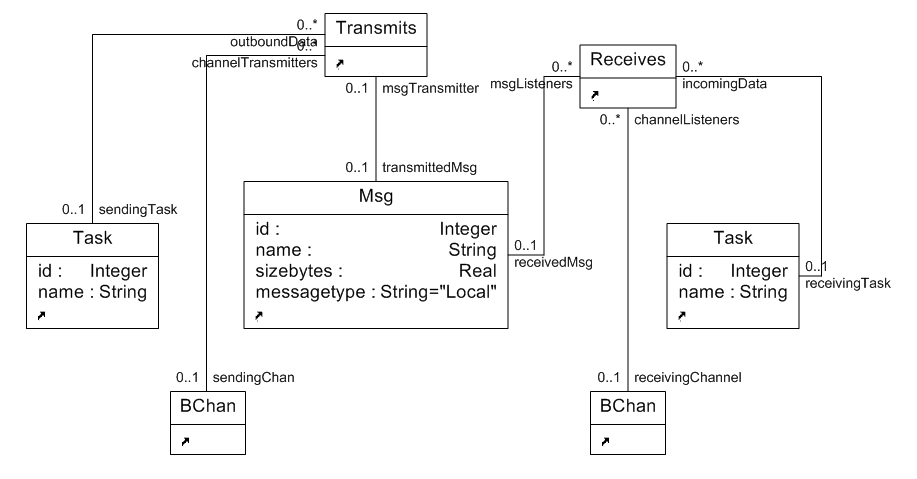
\includegraphics[width=0.8\columnwidth]{figures/tran_rcv.png}
    \caption{Transmit and receive relations in ESMoL Abstract, 
representing the endpoints of data transfers between nodes.}
    \label{fig:trnrcv_meta}
\end{figure}

\begin{figure}
\centering
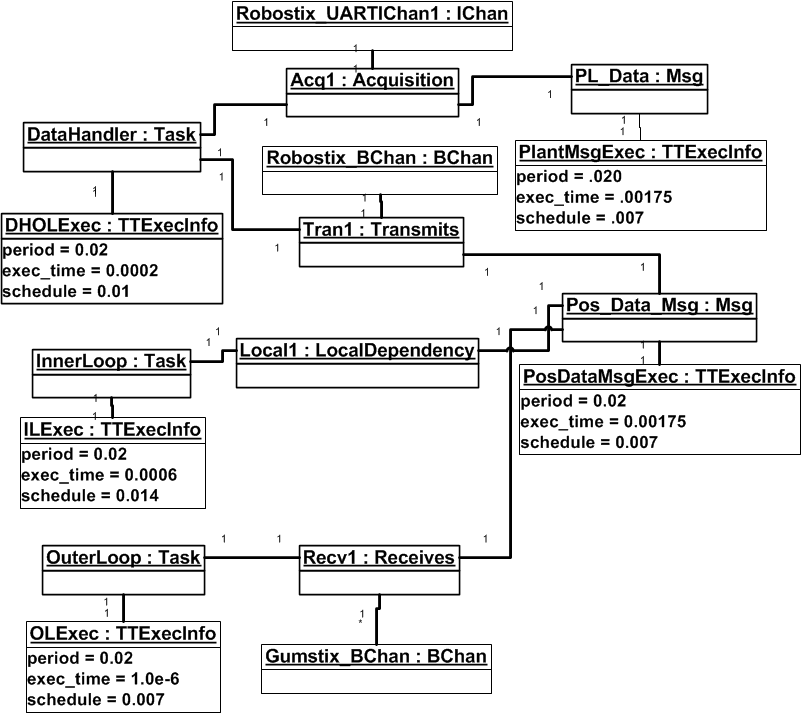
\includegraphics[width=0.85\columnwidth]{figures/msg_struct.png}
    \caption{Object diagram from part of the message structure example
from Figs. \ref{fig:qr_log_arch} and \ref{fig:qr_hw_mapping}. }
    \label{fig:msg_sched}
\end{figure}

\textbf{Bus Transfers: Data Movement Between Nodes}
Bus transfers are slightly more complicated, as they involve two or more
endpoints.  Table \ref{tab:transmit} and Fig.
\ref{fig:trnrcv_meta} contain the details. The send and receive relations
are modeled separately as they have different cardinalities (one sender 
and possibly multiple receivers).  The platform-specific code generators
produce separate files for each processor (recall that the network
may be heterogeneous). Fig. \ref{fig:msg_sched} shows an 
example of the objects and parameters based on our
design example.  The object diagram is an instance of the 
abstract language constructs shown in Figs. \ref{fig:acq_meta}, 
\ref{fig:localdep_meta}, and \ref{fig:trnrcv_meta}. 
The diagram depicts ESMoL\_Abstract relations of type
\emph{Acquisition}, \emph{LocalDependency}, \emph{Transmits}, 
and \emph{Receives}.  These objects are
involved in collecting position data from the sensors (task \emph{DataHandler}
from data channel \emph{Robostix\_UARTChan1}), and then redistributing it 
locally to the InnerLoop task as well as remotely to the \emph{OuterLoop} task
through the bus channel interfaces on the Robostix and Gumstix nodes.

\subsection{Stage 2 Transformation Outputs: Analysis Models and Code}

\begin{figure}
\centering
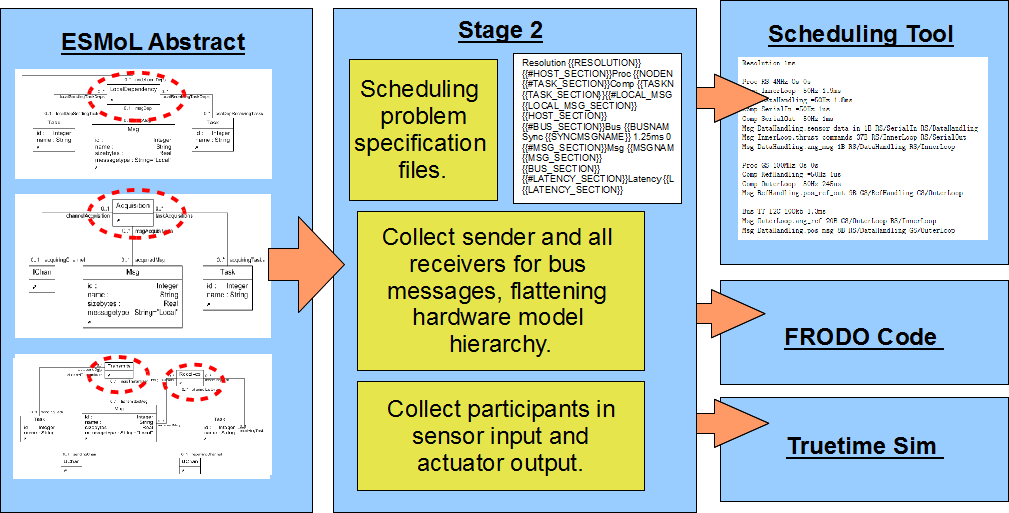
\includegraphics[width=0.95\columnwidth]{figures/stage2.png}
   \caption{Stage 2 Interpreter.}
   \label{fig:stage2}
\end{figure}

Stage 2 generates analysis models and code from ESMoL\_Abstract models
(Fig. \ref{fig:stage2}).  To perform 
the actual generation of analysis models and code, we use 
the CTemplate library\cite{tools:ctemplate} called from C++.
The current Stage 2 interpreter is generally used in a particular sequence:

\begin{enumerate}
 \item Generation of the scheduler specification.
 \item Creation of a TrueTime simulation model.
 \item Generation of platform-specific code using the FRODO virtual machine API.
\end{enumerate}

We will cover details for generation of scheduling problem 
specifications and FRODO-specific code.  The TrueTime code generation
is documented elsewhere\cite{modeling:truetime}.

\subsubsection*{Scheduling Problem Generation}
\label{section:schedules}

\begin{figure}
\centering
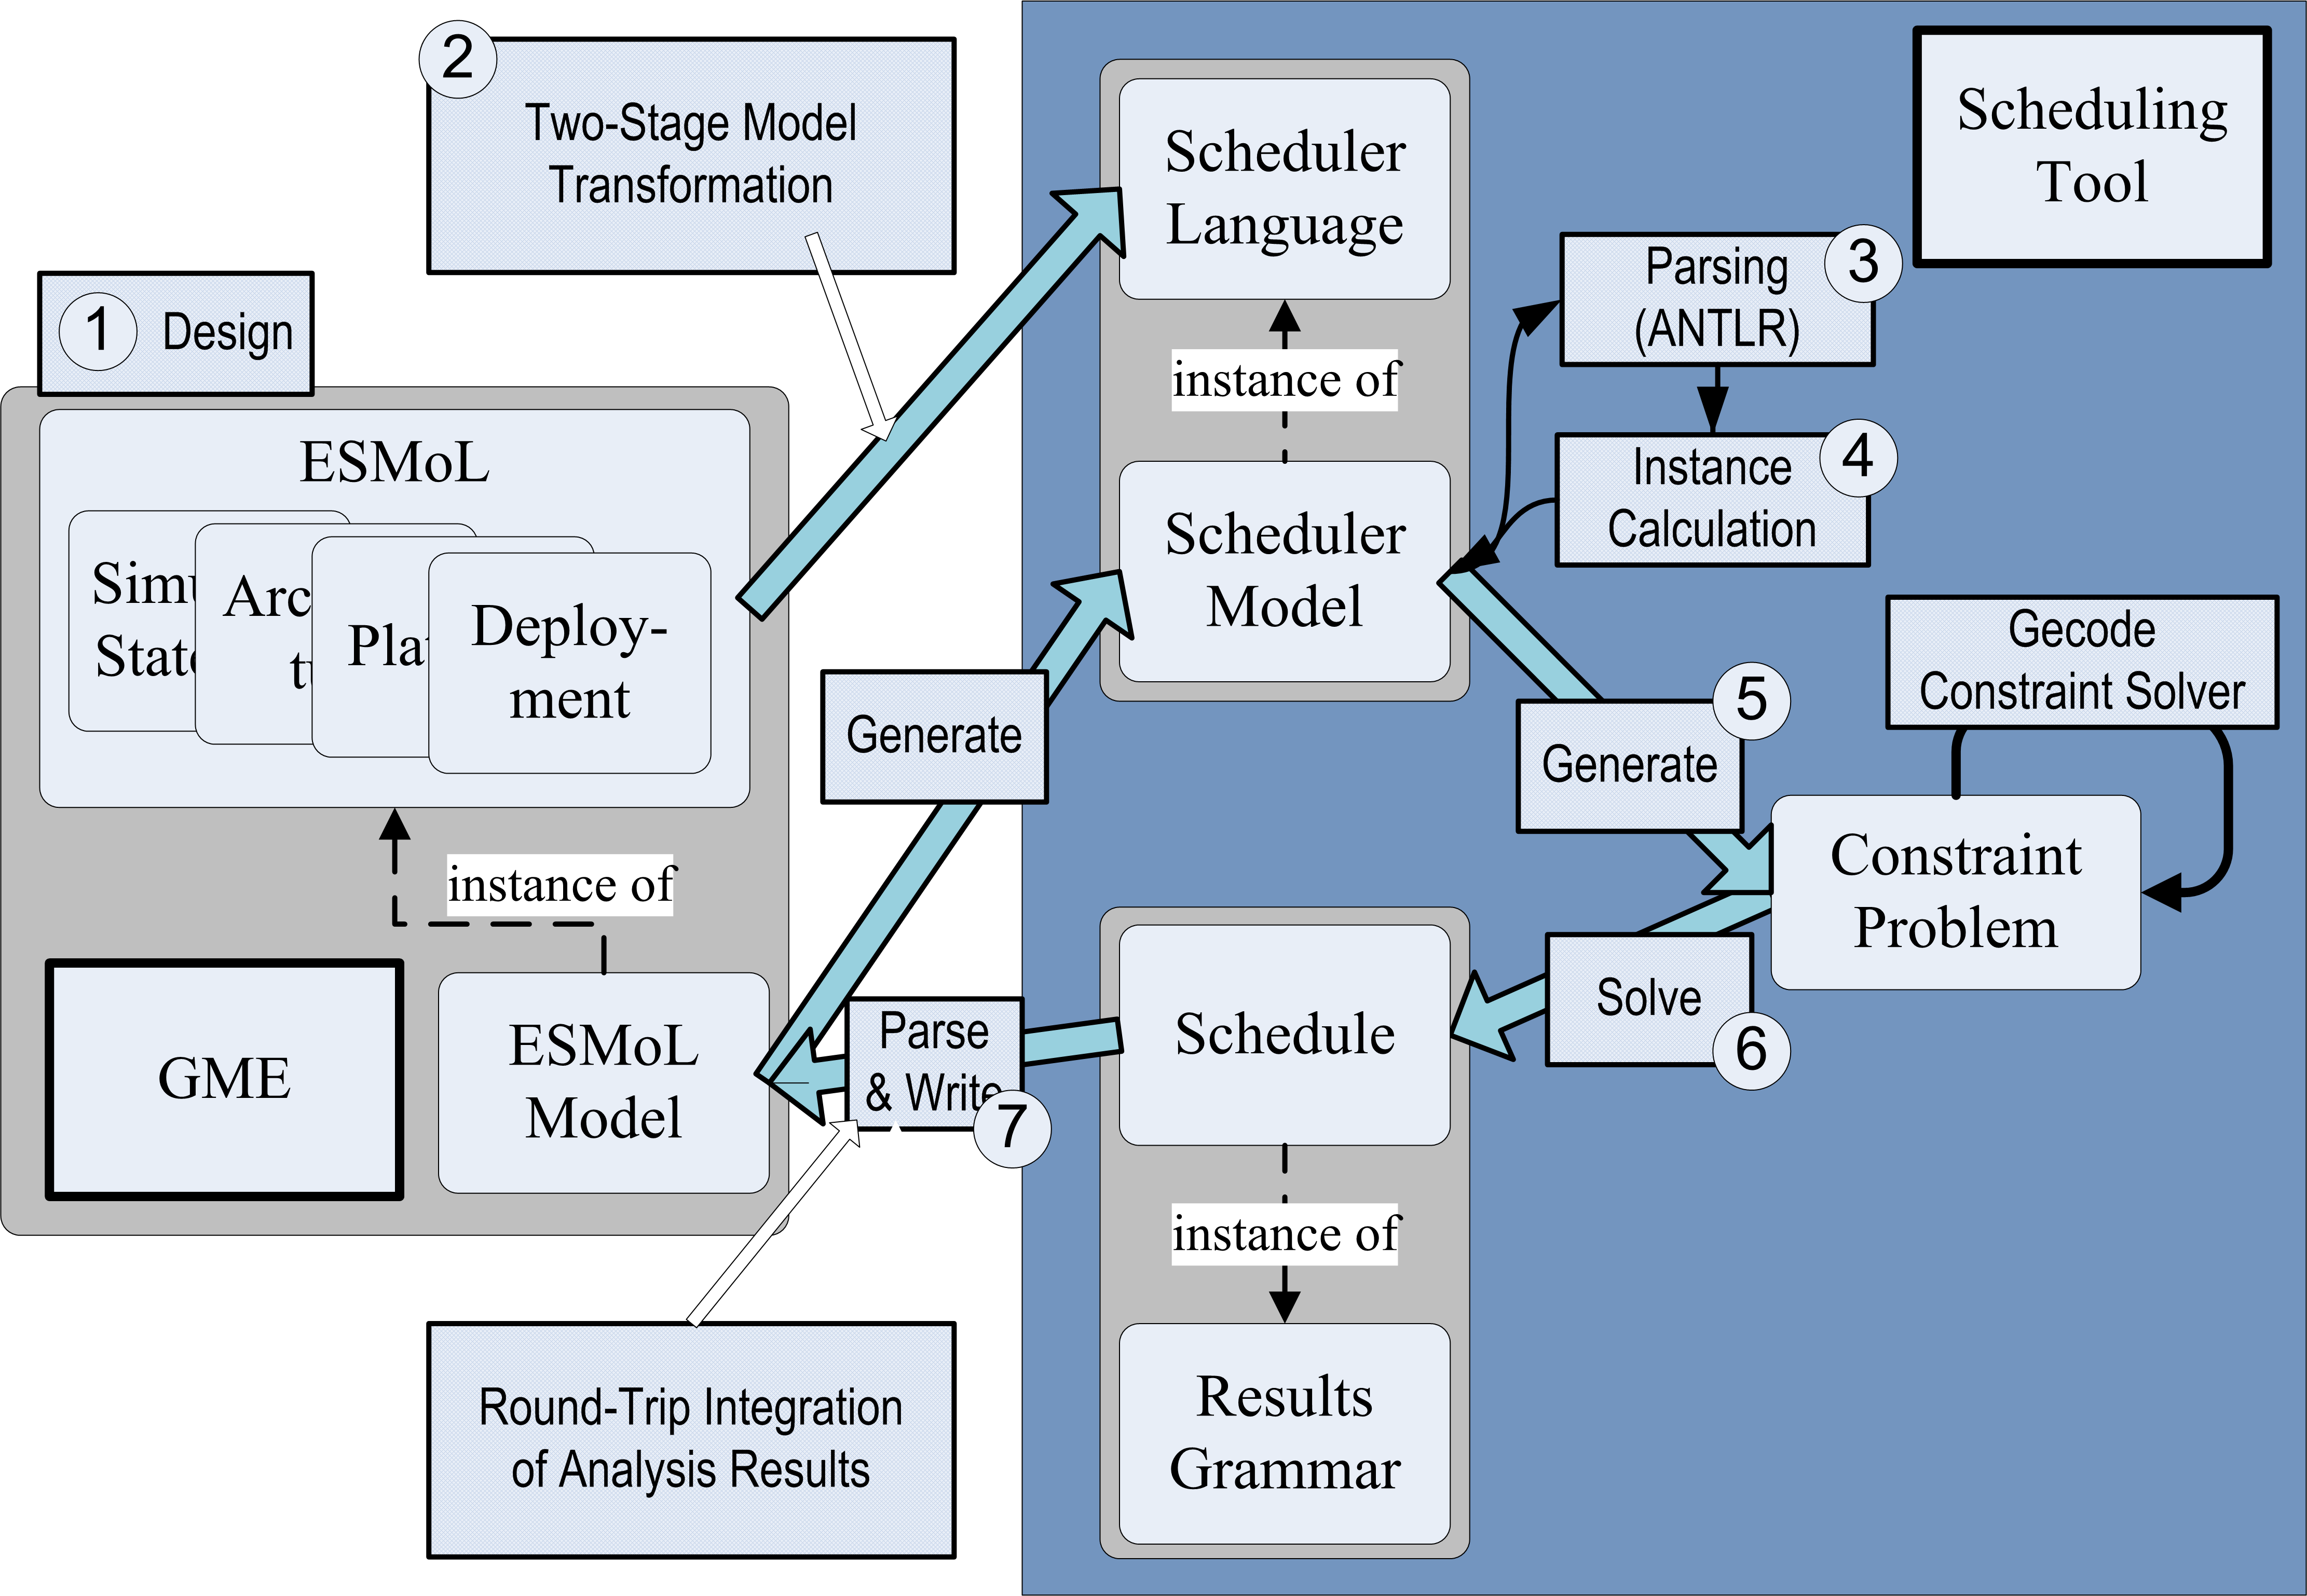
\includegraphics[width=0.85\columnwidth]{figures/sched_integration.png}
    \caption{Integration of the scheduling model by round-trip structural transformation between the language 
of the modeling tools and the analysis language.}
    \label{fig:sched_int}
\end{figure}

The control design models provide task period configurations, and 
either profiling or static analysis provides worst-case 
execution time parameters for each component instance.  
Data transfer rates and overhead parameters for communication
buses are stored in the platform model. \cite{sched:analysis}
describes the mapping of model structure, execution information,
and platform parameters into actual constraint model details, 
extending earlier work on constraint-based schedule 
calculation\cite{sched:offline}. The Gecode constraint programming
tool \cite{tools:gecode} solves these constraints for task release and
message transfer times on the time-triggered platform. The scheduling process
guarantees that the implementation meets the timing requirements 
required by the control design process.

Fig. \ref{fig:sched_int} portrays the steps a 
model transformation takes while distilling details from ESMoL and 
creating a scheduling problem model whose 
syntax represents the proper sets of behaviors.  If the
schedule is feasible, task and message release 
time results are fed back into the ESMoL model 
as configuration parameters.  We describe the steps
indicated in the diagram here:

\begin{enumerate}
 \item We start with a design model specified using ESMoL.
 \item The two-stage transformation converts the model to an equivalent model in ESMoL\_Abstract, and then invokes the templates to generate a scheduling problem specification.
 \item We invoke the scheduling tool, which performs the following steps:
 
 \begin{enumerate}
 \item Parses the problem specification to import the model into the constraint generation environment.
 \item Calculates the hyperperiod length to determine the number of instances required for each task and message.
 \item Translates task and message instance relationships into constraints in Gecode (as described in \cite{sched:analysis}).
 \item Solves the constraint problem, possibly indicating infeasibility.  
 \item If a valid schedule results, it is written out to a file.
 \end{enumerate}
 \item The results are imported into the ESMoL model and written to the appropriate objects.
\end{enumerate}

Table \ref{code:qr_spec} contains the distributed schedule 
specification for our quadrotor example, including the following elements:

\begin{itemize}
\item {\bf Resolution} (seconds) specifies the size of a single processing tick for the global schedule.  This should correspond to the largest measurable time tick (quantum) of the processors in the network.  All tasks and messages in the schedule timeline are discretized to this resolution.
\item {\bf Proc} specifies a processing node.  Parameters are name, processor speed (Hz), and message send/receive overhead times (these default to zero seconds if unspecified).  Processor names must be unique.
\item {\bf Comp} (or task) belongs to the most recently specified processor.  A component is characterized by its name, period, and worst-case execution time (WCET) (both in seconds).  We do not address the manner in which the WCET is to be obtained.
\item {\bf Bus} specifies a bus object, characterized by name, transfer speed (bits per second), and transfer overhead (also in seconds).
\item {\bf Msg} includes a name, byte length, sending task, and list of receiving tasks.
\end{itemize}

%\begin{framed}
%\lstset{basicstyle=\small,frame=none,label=schedspec,caption=Scheduling problem specification.}

%\begin{lstlisting}
%Resolution 2us

%Proc P1 100MHz 50us 10us
%Task T1 =50Hz 8us
%Task T2 =100Hz 10us

%Proc P2 100MHz 40us 12us
%Task T1 =50Hz 10us
%Task T2 =100Hz 10us

%Proc P3 100MHz 50us 12us
%Task T1 =25Hz 10us
%Task T2 =50Hz 5us

%Bus B12 1Mb 0us
%Msg M1 16B P1/T1 P2/T1

%Bus B23 1Mb 0us
%Msg M2 2B  P2/T1 P3/T1
%Msg M3 4B  P3/T2 P2/T2

%Latency 35us P1/T1 P2/T1
% Latency loop
%Latency 100us P2/T1 P2/T2
%\end{lstlisting}
%\end{framed}

Task and message names are unique only within 
their scope (processor or bus, respectively).  When used 
in other scopes they are qualified with their scope 
as shown (e.g. P3/T1). The timing constraints include 
the various platform overhead parameters.  For example, 
once the message length is converted from bytes to time on 
the bus, we add the transfer overhead to represent the 
setup time for the particular protocol.  Engineers 
must measure or estimate platform behavioral parameters 
and include them in models for the 
platform\cite{modeling:platform}.

\begin{table*}
\centering
%\begin{tabular}{@{\extracolsep{\fill}}| l |}
%\hline
\begin{alltt}
Resolution 1ms

Proc RS 4MHz 0s 0s
Comp InnerLoop =50Hz 1.9ms
Comp DataHandling =50Hz 1.8ms
Comp SerialIn =50Hz 1us
Comp SerialOut =50Hz 1ms
Msg DataHandling.sensor_data_in 1B RS/SerialIn RS/DataHandling 
Msg InnerLoop.thrust_commands 37B RS/InnerLoop RS/SerialOut
Msg DataHandling.ang_msg 1B RS/DataHandling RS/InnerLoop 

Proc GS 100MHz 0s 0s
Comp RefHandling =50Hz 1us
Comp OuterLoop =50Hz 245us
Msg RefHandling.pos_ref_out 9B GS/RefHandling GS/OuterLoop 

Bus TT_I2C 100kb 1.3ms
Msg OuterLoop.ang_ref 20B GS/OuterLoop RS/InnerLoop 
Msg DataHandling.pos_msg 8B RS/DataHandling GS/OuterLoop 
\end{alltt}
\caption{Scheduling spec for the Quadrotor example.}
\label{code:qr_spec}
%\end{tabular}
\end{table*}

\begin{table*}
\centering
\begin{alltt}
\scriptsize
Resolution \{\{RESOLUTION\}\}

\{\{\#HOST_SECTION\}\}Proc \{\{NODENAME\}\} \{\{NODEFREQ\}\} \{\{SENDOHD\}\} \{\{RECVOHD\}\}
\{\{\#TASK_SECTION\}\}Comp \{\{TASKNAME\}\} =\{\{FREQUENCY\}\} \{\{WCEXECTIME\}\}
\{\{\/TASK_SECTION\}\}\{\{\#LOCAL_MSG_SECTION\}\}Msg \{\{MSGNAME\}\} \{\{MSGSIZE\}\} \{\{SENDTASK\}\} \{\{RECVTASKS\}\}
\{\{\/LOCAL_MSG_SECTION\}\}
\{\{\/HOST_SECTION\}\}
\{\{\#BUS_SECTION\}\}Bus \{\{BUSNAME\}\} \{\{BUSRATE\}\} \{\{SETUPTIME\}\} \{\{\#BUS_HOST_SECTION\}\}\{\{NODENAME\}\} \{\{\/BUS_HOST_SECTION\}\}
\{\{\#MSG_SECTION\}\}Msg \{\{MSGNAME\}\} \{\{MSGSIZE\}\} \{\{SENDTASK\}\} \{\{RECVTASKS\}\}
\{\{\/MSG_SECTION\}\}
\{\{\/BUS_SECTION\}\}
\{\{\#LATENCY_SECTION\}\}Latency \{\{LATENCY\}\} \{\{SENDTASK\}\} \{\{RECVTASK\}\}
\{\{\/LATENCY_SECTION\}\}
\end{alltt}
\caption{Stage 2 Interpreter Template for the Scheduling Specification}
\label{code:sched_templ}
\end{table*}

Scheduling specifications are created in the Stage 2 interpreter from
the template shown in Table \ref{code:sched_templ}.
The Stage 2 scheduler generation logic traverses the 
ESMoL\_Abstract model and fills in the structures
which are used to fill in the template when the 
CTemplate generator is invoked.  
In CTemplate, each \verb${{#...}} {{/...}}$ tag pair delimits a 
section which can be repeated by filling in the proper data 
structure in the code.  The other tags \verb${{...}}$ are 
replaced by the string specified in the generation code. 

Producing the \emph{Proc} and \emph{Comp} lines from the model 
API is straightforward as the output mirrors the model
hierarchy, so these lines require only simple traversals 
of the model.  Each generated line uses parameters 
from the respective model object to fill in the blanks.  
The parameters are shown only in the 
generated output, though the object diagram in 
Fig. \ref{fig:msg_sched} illustrates a good example 
of parameter layout and disposition.  In order to produce 
each \emph{Msg} line, many relations must be collected (as shown 
in Table \ref{tab:localdeps} and Fig. \ref{fig:localdep_meta} ) 
and distilled into the right relationships.  This requires 
more complex traversal code often involving multiple passes
through the model objects.   
To write a new generator similar to this one, the developer uses the 
interpreter API and the transformed abstract syntax graph model.  
In the abstract language traversal we collect the 
\emph{LocalDependency} objects and filter them by processor. 
Each \emph{LocalDependency} object contains all of the 
information necessary to fill out the parameters in 
the template and create a new Msg line in the
scheduler specification file (within the proper \emph{Proc} scope).

While we do not list here the details related to 
the solution of scheduling specifications, it may be useful 
to document some of the scheduler limitations.  More 
details regarding these limitations may be found in 
\cite{sched:analysis}.

\begin{itemize}
\item We do not support preemptive scheduling of tasks or messages, 
as our runtime provides conflict-free task execution and data
communication during nominal operation.
\item The overhead parameters may be an overly simplistic model for some cases. Each processor and bus 
pair may have different parameters, depending on the bus type and the protocol used.
\item We do not perform optimization on the schedule, so performance cost functions are not taken into 
account.  For control problems where the execution time changes yield irregular performance changes, this 
is a more serious issue (see for example \cite{control:scheduling} ).
\end{itemize}

\subsubsection*{Platform-Specific Code Generation}

Time-triggered execution requires configuration with the computed 
cyclic schedule.  Code generated for the virtual machine 
conforms to a particular synchronous execution strategy -- each 
task reads its input variables, invokes its component functions, and 
writes its output variables.  The schedule calculation assumes logical
execution time semantics, where task input data is ready before 
task release, and output data is not assumed ready before the task 
completes\cite{modeling:giotto3}. Data structures describe the 
invocation times and configuration parameters for tasks and messages
on each processor.   
Each message configuration instance also includes local buffer addresses 
where the timed communication controller in the virtual machine 
can store incoming and outgoing message data.  

%\scriptsize
\begin{table*}
\centering
\begin{alltt}
////////////////////////////// SCHEDULE TABLE ///////////////////////////////

portTickType hp_len = 20;

task\_entry tasks[] = \{
   \{ DataHandling, "DataHandling", 4, 0\},
   \{ InnerLoop, "InnerLoop", 9, 0\},
   \{NULL, NULL, 0, 0\}
\}\;

msg\_entry msgs[] = \{
   \{ 1, MSG\_DIR\_RECV, sizeof( OuterLoop\_ang\_ref ), 
      (portCHAR *) \& OuterLoop\_ang\_ref, 
      (portCHAR *) OuterLoop_ang\_ref\_c, 7, 0, 0\},
   \{ 2, MSG\_DIR\_SEND, sizeof( DataHandling\_pos\_msg ), 
      (portCHAR *) \& DataHandling\_pos\_msg, 
      (portCHAR *) DataHandling\_pos\_msg\_c, 11, 0, 0\},
   \{ -1, 0, 0, NULL, NULL, 0, 0, 0\}
\}\;

per\_entry pers[] = \{
   \{ 1, "UART", IN, 0, 0, sizeof( DataHandling\_sensor\_data\_in ), 
      (portCHAR *) \& DataHandling\_sensor\_data\_in, 
      (portCHAR *) DataHandling\_sensor\_data\_in\_c, 2, NULL, 0, 0\},
   \{ 2, "UART", OUT, 0, 0, sizeof( InnerLoop\_thrust\_commands ), 
      (portCHAR *) \& InnerLoop\_thrust\_commands, 
      (portCHAR *) InnerLoop\_thrust\_commands\_c, 14, NULL, 0, 0\},
   \{ -1, NULL, 0, 0, 0, 0, NULL, NULL, 0, NULL, 0, 0 \}
\}\;

\end{alltt}
\caption{Generated code for the task wrappers and schedule structures of the Quadrotor model.}
\label{code:frodo_gen}
\end{table*}

%\scriptsize
\begin{table*}
\centering
\begin{alltt}
////////////////////////////// SCHEDULE TABLE ///////////////////////////////

portTickType hp_len = \{\{NODE_hyperperiod\}\};

\{\{\#SCHEDULE_SECTION\}\}
task\_entry tasks[] = \{
\{\{\#TASK\}\}
   \{ \{\{TASK_name\}\}, "\{\{TASK_name\}\}", \{\{TASK\_startTime\}\}, 0\},\{\{\/TASK\}\}
   \{NULL, NULL, 0, 0\}
\}\;

msg\_entry msgs[] = \{
\{\{\#MESSAGE\_NAME\}\}
   \{ \{\{MESSAGE\_index\}\}, \{\{MESSAGE\_sendreceive\}\}, sizeof( \{\{MESSAGE\_name\}\} ), 
         (portCHAR *) \& \{\{MESSAGE\_name\}\}, 
         (portCHAR *) \& \{\{MESSAGE\_name\}\}\_c, \{\{MESSAGE\_startTime\}\}, 
         pdFALSE\},
\{\{\/MESSAGE\_NAME\}\}
   \{ -1, 0, 0, NULL, NULL, 0, 0\}
\}\;

per\_entry pers[] = \{
\{\{\#PER_NAME\}\}
   \{ \{\{PER\_index\}\}, "\{\{PER\_type\}\}", 
         \{\{PER\_way\}\}, 0, \{\{PER\_pin\_number\}\}, sizeof( \{\{PER\_name\}\} ), 
         (portCHAR *) \& \{\{PER\_name\}\}, 
         (portCHAR *) \& \{\{PER\_name\}\}\_c, 
         \{\{PER\_startTime\}\}, NULL\}, 
\{\{\/PER_NAME\}\}
   \{ -1, NULL, 0, 0, 0, 0, NULL, NULL, 0, NULL \}
\}\;
\{\{\/SCHEDULE_SECTION\}\}

\end{alltt}
\caption{Template for the virtual machine task wrapper code. The Stage 2 FRODO interpreter invokes
this template to create the wrapper code shown in Table \ref{code:frodo_gen}.}
\label{code:frodo_templ}
\end{table*}

The generated code for the Quadrotor model in Table 
\ref{code:frodo_gen} was produced from the template description
for the platform-specific code generator in Table \ref{code:frodo_templ}.
The FRODO virtual machine generation template brings together all of the
ESMoL\_Abstract relations described in the earlier section.  
The template and generated code
segment above correspond to the second-stage 
interpreter that creates the static schedule
structures used by the virtual machine.  The tasks, 
messages, and peripherals listed here come from the 
\emph{Acquisition}, \emph{Actuation}, \emph{Transmit}, and 
\emph{Receive} relation objects.  The various connected 
objects are sorted according to schedule time, and then the 
template instantiation uses the object parameters
to create the tables in a manner similar to that 
described for the scheduler specification generation above.  
The \emph{LocalDependency} relations do not appear in this template.  
The scheduler creates constraints that must be
satisfied for each local dependency, but local message transfers take place automatically in shared memory as tasks write to and read from processor-local message structures.  Therefore, any valid task and message
schedule will satisfy them.  In a different part of the FRODO template, the
local dependencies determine which message fields must be used as
arguments to the component function calls (not shown here).

\section{Synchronous Semantics}

We will briefly present a formal argument for the preservation of synchronous
Simulink block firing orders as we use the Simulink blocks to define software
components, their deployment to the hardware, and impose a time-triggered 
execution schedule on the design.  Our semantic argument is only valid for
synchronous data flow (SDF) specifications.  We do not claim to represent the
full generality of Simulink specifications, rather we restrict ourselves to
dataflow graphs without conditional execution.  Our graphs must contain only
tasks that execute in periodic, discrete time,  have no
delay-free loops, all delay elements must be initialized with a data token,
and initial block firing orders must include the outputs of the delay elements 
This final assumption can be satisfied by considering the outputs of the delay elements as additional inputs to the component.  Then all dependent blocks will be able to fire as early as necessary in the schedule.  Our restrictions on 
execution are consistent with those 
required by the Mathworks Real-Time Workshop Embedded Coder product, 
which forces models to have fixed-step execution and task periods 
harmonic with the configured time step size for code generation.

Consider a synchronous acyclic graph $\mathbb{G}=(V,E)$ representing the 
connectivity of a Simulink dataflow model, where edges abstract the transfer 
of data between blocks (without the data type information, data capacity, or 
multiplicity). Let $exec: \mathbb{G} \rightarrow \mathbb{R}$ represent the
task duration for vertices (obtained by analysis or measurement), and the
communication message transfer time for edges.

Let $C_V \subseteq V \times \mathbb{Z}^{|V|}$ be the set of all possibly 
concurrent firing orders for the blocks represented by the set $V$ which 
respect the partial order specified by the edge set $E$ (i.e. $(v_1, v_2) \in E \Rightarrow c(v_1) < c(v_2) \forall c \in C_V$ where the 
pairs in $c$ are interpreted as functions on $V$).  Note that $C_V$ 
should only be taken up to isomorphism, eliminating orderings that are 
equivalent.

Consider the synchronous execution of $\mathbb{G}$, where the full graph is 
executed on a periodic schedule at instants 
$\{T_s k\}, (k = 0,1,\ldots,\infty)$, and completes each execution before the 
next cycle.  For embedded code generation, Simulink requires models to 
execute with fixed-step semantics, so
this is not an overly strong restriction.

Next, we allow manipulations of the dataflow graph $\mathbb{G}$ as follows:
Let $\mathbb{G}' \subseteq \mathbb{G}$ be a subgraph.  Assume that $\mathbb{G}'=(V',E')$ represents a well-formed functional dataflow.   Let $C_{V'} \subseteq V' \times \mathbb{Z}^{|V'|}$ be a set of possible orderings for $V'$ created by
restricting $C_V$ to the vertex set $V'$.  All orderings in $C_{V'}$ are also
valid in $C_V$, if we adjoin proper orderings from $C_{V-V'}$.  All orderings 
in $C_{V'}$ are also synchronous orderings, as they respect the partial order 
defined by $\mathbb{G}'$.  We can also
continue this construction for products.  Let $\mathbb{G}' \subseteq \mathbb{G}$ and $\mathbb{G}'' \subseteq \mathbb{G}$, where we uniquely identify the vertex
sets $V'$ and $V''$ so that $V' \cap V'' = \emptyset$.  Then for 
$\mathbb{G}' \times \mathbb{G}''$ we have $C_{V'} \times C_{V''}$.  
Considering the concurrent execution of $\mathbb{G}'$ and $\mathbb{G}''$, both
graphs execute synchronously if executed according to an order from
$C_{V'} \times C_{V''}$.

Let $\mathbb{G}_{s_1}, \ldots, \mathbb{G}_{s_I}$ be subgraphs of a Simulink dataflow $\mathbb{G}$.
These represent ESMoL-specified dataflows.  Let $\mathbb{G}_s = \times_{i \in [1,I]} \mathbb{G}_{s_i}$ where each vertex $v \in V_s$ is given a unique identity as above.
Consider the product of the restricted orderings $C_{V_s} = \times_{i \in [1,I]} (V_{s_i} \times \mathbb{Z}^{|V_{s_i}|})$.  Then the specified dataflow $\mathbb{G}$ is synchronous if executed according to an order from $C_{V_s}$.

Consider the following partitions on $\mathbb{G}_s$:

Let $C_p: V_s \rightarrow [1,P]$ assign component blocks to physical processors.

Let $C_T: V_s \rightarrow [1,N]$ assign components to computational tasks.  We need to ensure that all components belonging to the same task also belong to the same processor ($\forall n \in [1,N], \exists p \in [1,P] : \{v \in V_s | C_T(v)=n\} \Rightarrow \{v | C_P(v) = p\}$.

Let $\{b_1, \ldots, b_B\}$ be a set of physical communication buses, $\{t_1, \ldots, t_N\}$ be the set of tasks, and $\{p_1, \ldots, p_P\}$ be the set of 
physical processors.  Let $B_E =  \{b_1, \ldots, b_B\} \cup \{t_1, \ldots, t_N\} \cup \{p_1, \ldots, p_P\}$.  Let $C_E: E_S \rightarrow B_E$ represent the 
communication mode for each data message represented by a graph edge.  
Data can travel remotely (via a data bus $b_i$) or locally in shared memory 
(between components within a task $t_j$ or between tasks on a processor $p_k$).

Let $D \subseteq C_{V_s}$ be the subset of the orderings for $\mathbb{G}_s$
restricted such that if $o \in D$, then 

\begin{equation*}
\forall v_1,v_2 \in V_s, C_P(v_1) = C_P(v_2) \Rightarrow o(v_1) \neq o(v_2)
\end{equation*}
  
$D$ is the restriction of the 
synchronous orderings on $V_s$ to the hardware partitioning, where two vertices cannot have
the same order if they share a resource.  Note that if the design is not
schedulable, $D$ will not exist.

Finally, consider the schedule.  Let $S: \mathbb{G}_s \rightarrow \mathbb{R}^{|V_s|+|E_s|}$ represent start times for all elements of the dataflow graph $\mathbb{G}_s$. 

Let $D' \subseteq D$ satisfy ($\forall o' \in D'$):

\begin{gather*}
\forall v_1, v_2 \in V_s, e = (v_1, v_2) \in E_s \wedge C_P(v_1) \neq C_P(v_2) \\
\Rightarrow S(v_2) > S(v_1) + exec(v_1) + exec(e) \wedge o'(v_2) > o'(v_1)
\end{gather*}.  

If two components have a dependency through a remote message, then their start times are constrained by the start time of $v_1$, the duration of $v_1$, and the duration of the message represented by the edge $e$. This models the logical execution time semantics of time-triggered execution.  Note that the addition of the edge time may push the order values farther apart by allowing other tasks to execute during the data transfer time, so the reduction involved in $D'$ may be significant.  Again, we assume that the model is schedulable.

Since the final set of orderings $D'$ was constructed by reduction from the initial set of orderings $C_V$, any scheduling policy for ESMoL that enforces the 
constraints and partitionings shown above will maintain the synchronous 
semantics of the original Simulink model if the ESMoL model is schedulable.
Note that we have not dealt with delays.  The scheduling tool described in 
Porter et al\cite{sched:analysis} conforms to the constraints as described, if
combined with the Stage1 logic to create local dependencies for transitive remote connections as described above.  Unfortunately, the scheduler does not enforce end-to-end latencies well, an issue which the authors are currenlty working to address.

\section{Evaluation}
\label{section:devflow}

Our approach for creating high-confidence designs 
varies somewhat from the traditional V-diagram 
development model (see Fig. \ref{fig:vdiagram}).  In the
traditional model we move down the V, refining designs 
as we proceed, with the level of integration increasing 
as the project progresses.  We recognize that system integration 
is often the most costly and difficult part of development.
Lessons learned during integration frequently occur 
too late to benefit project decision-making.  We aim to 
automate much of the integration work, and therefore shorten 
design cycles.  Beyond that, we want to enable feedback of 
models and analysis results from later design stages back 
to earlier design cycles (along the dashed lines in the 
conceptual diagram) to facilitate rapid rework if necessary.  The
goal is that the overall project can rapidly move towards 
a correct implementation that most accurately reflects our 
current understanding of the design problem.

\begin{figure}
   \centering
   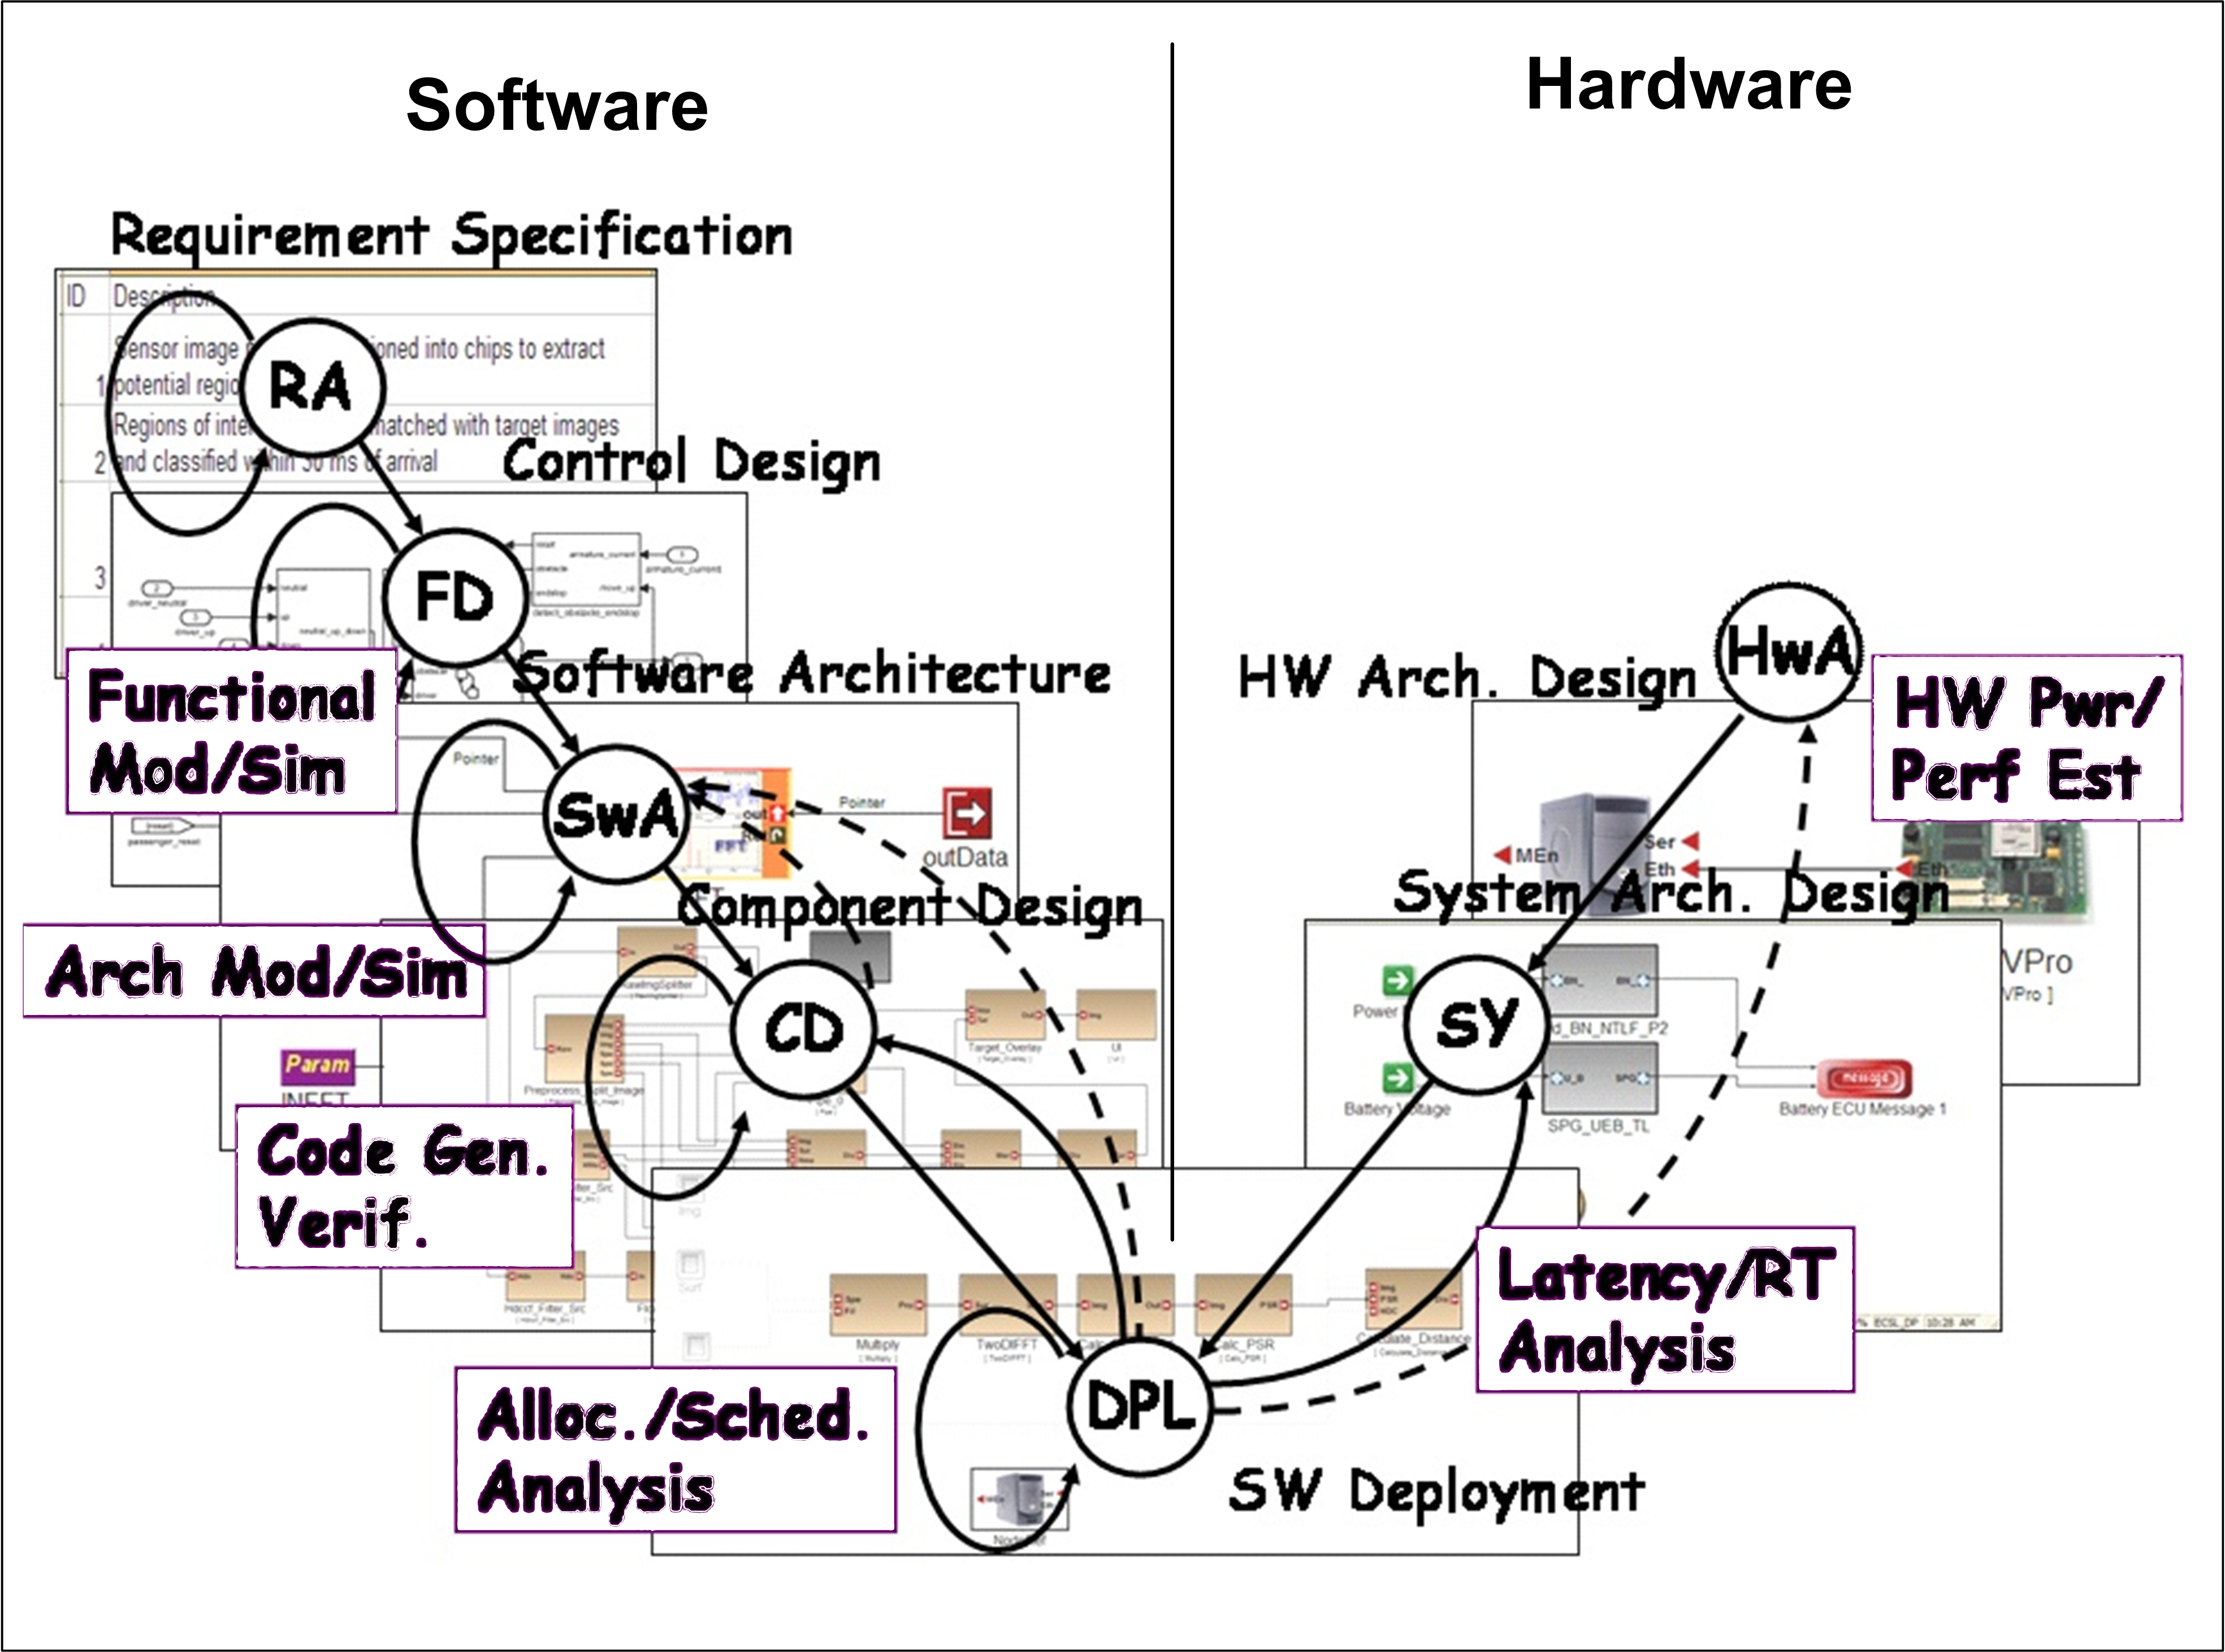
\includegraphics[width=0.85\columnwidth]{figures/vdiagram.png}
   \caption{Conceptual development flow supported by the tool chain.}
   \label{fig:vdiagram}
\end{figure}

Our case study covers the incremental development of software for 
the Starmac quadrotor aircraft \cite{quad:starmac,quad:starmacdyn}.
We deployed our software to the same hardware as the Starmac controller
(with the exception of our internal $I^2C$ link, where the Starmac design
used a UART), and tested in a
hardware-in-the-loop environment which simulated the Starmac
dynamics.  Specifically, we conducted three development phases
(each with a corresponding set of design models), each of which 
successively refined the design while preserving the component
structure:

\begin{enumerate}
\item {\bf Communications Test:} We designed and deployed a shell
of the controller architecture, where the software controller components
received and sent messages of the proper size, but the system functions only
copied data from the input ports to the output ports of each component.  The 
Mathworks xPC Target Hardware-in-the-Loop (HIL) simulator injected known 
data patterns into the
deployed dataflow implementation to ensure that all data paths were valid
given the configured schedule.
\item {\bf Quad Integrator Test:} We designed and deployed a simplified
version of the quadrotor which acted only along a single axis of motion,
removing the rotational dynamics.  We were able to validate our control
design approach (see \cite{pass:validation}), and determine a method for 
gain adjustments required for stable operation of the deployed controller. 
\item {\bf Quadrotor Test:} The final phase evaluated the full quadrotor
dynamics and controller implementation.  We tested trajectory tracking 
with the full platform delay effects.
\end{enumerate}

Each of the three development phases answers a set of questions regarding
the correctness of the design under nominal operating conditions:

\begin{itemize}
\item {\bf Communications Test:}
\begin{enumerate}
\item Is the hardware configuration valid for this software configuration?
\item Does our deployment mapping communicate the right amounts of data round trip?
\item Does the configured schedule avoid communication conflicts?
\item Is data corrupted by the communication protocols or software?
\item How much delay is introduced by the configured schedule?
\end{enumerate}
\item {\bf Quad Integrator Test:}
\begin{enumerate}
\item Does our methodology for selecting stabilizing gains for the control
loops adequately handle the schedule delay introduced by data buffering,
network communication, and the calculated schedule?
\item Is our sampling process sufficient for the platform and essential 
control architecture?
\item Are there any numerical problems that arise in our functional dataflow implementation considering normal input value ranges?
\end{enumerate}
\item {\bf Quadrotor Test:}
\begin{enumerate}
\item Given the additional functions and dimensions in the dataflow, can we still properly answer all of the questions from the previous phase?
\item Does the full configuration track a reference trajectory?
\end{enumerate}
\end{itemize}

Fig. \ref{fig:hil_setup} is a conceptual depiction of our evaluation 
environment.  The Mathworks xPC Target simulation software runs on a generic small-form-factor PC, with ethernet for configuration and data collection.  The xPC system contains an 8-port RS-232 serial expansion card, which communicates with the controller hardware on one port.  The simulator and controller send sensor and actuator data back and forth on a single full-duplex serial link running at 57600 baud.  The controller hardware consists of two processor boards -- the Gumstix Linux board runs the \emph{OuterLoop} controller and the 
\emph{RefHandler} data input tasks.  The Gumstix board has access to an ethernet port, through which the host machine sends new controller software for both control boards.  We also use secure shell connections to start and stop the controller, and to monitor for error messages which are printed to the console. An internal $I^2C$ connection allows the two control boards to exchange sensor data and attitude control commands.  The Robostix AVR board runs the \emph{InnerLoop} attitude controller and the \emph{DataHandler} sensor data distribution component.  One Robostix UART device connects to the xPC simulator as described above.  Digital I/O pins allow the monitoring of timing information for the Robostix.  We embedded commands to toggle the I/O pins in the controller software, and connected the pins to the LogicPort logic probe.  The probe software shows timing traces for evaluating schedule operation (as in Fig. \ref{fig:sched_nodelays}). A software AVR simulator was also used to evaluate timing and stack usage for the software running on the AVR.  The Robostix board runs FreeRTOS.  A Windows virtual machine on the host PC runs the ESMoL modeling tools, logic probe display software, and Simulink which configures and compiles models for the xPC target software.  The Linux-based host itself runs the cross-compilers for the controller targets, and secure shell connections to the Gumstix board for status monitoring.

\begin{figure}
   \centering
   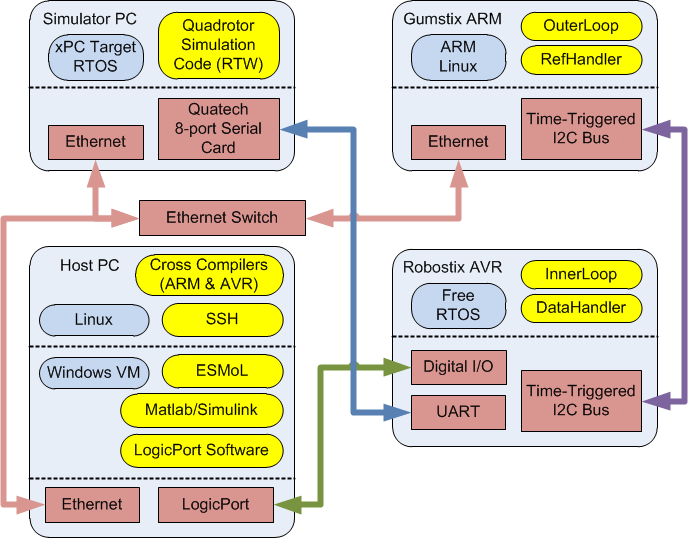
\includegraphics[width=0.85\columnwidth]{figures/hil_setup.png}
   \caption{Hardware in the Loop (HIL) evaluation configuration.}
   \label{fig:hil_setup}
\end{figure}

\subsection{Communications Test}

\begin{figure*}
\centering
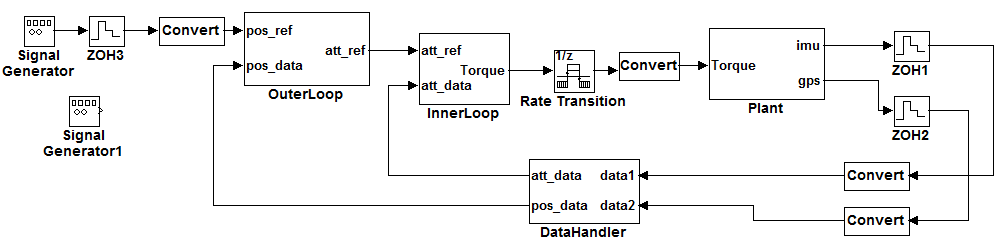
\includegraphics[width=0.9\columnwidth]{figures/comms_test.png}
    \caption{Communications test model.}
    \label{fig:comms_test_mdl}
\end{figure*}

\begin{figure*}
\centering
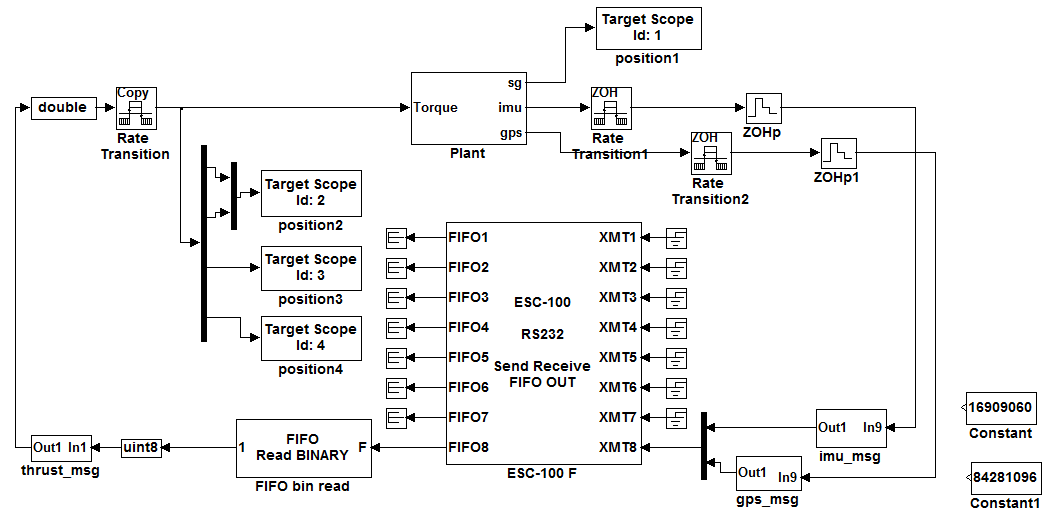
\includegraphics[width=0.9\columnwidth]{figures/comms_test_xpc.png}
    \caption{Communications test plant model using the Mathworks xPC Target.}
    \label{fig:comms_test_plant}
\end{figure*}

Fig. \ref{fig:comms_test_mdl} displays the simple model used to 
test data flow over the communication channels.  The blocks contain only
pass-through elements -- multiplexers, demultiplexers, and gains.  
With this model we verified that data flowed correctly through all of the
data paths in the system.  The \emph{InnerLoop}, \emph{OuterLoop},
and \emph{DataHandler} components were all realized in software from an
ESMoL model, and deployed to the hardware platform.  
The execution of the components is controlled by a simple time-triggered virtual machine that releases tasks and messages at pre-calculated time instants. 

The Mathworks xPC Target simulated the plant dynamics for this
test, which in this case amounted only to signal generators to create known
data for the simplified controller blocks, and scopes to visualize data received from the controller board.  We compared the input and output traces for
(delayed) equality (Fig. \ref{fig:comms_test_plant}).

During this phase we found problems with the $I^2C$ communications link.  The
scheduling and timed execution both required precise coordination to prevent
data corruption.  We also manually discovered a deadlock condition in our 
communications controller logic.  Increasing the speed of the $I^2C$ link from 
100 kbits/sec to 400 kbits/sec resolved both the scheduling problem and the
deadlock.

\subsection{Quad Integrator Model}

\begin{figure*}[thb]
\centering
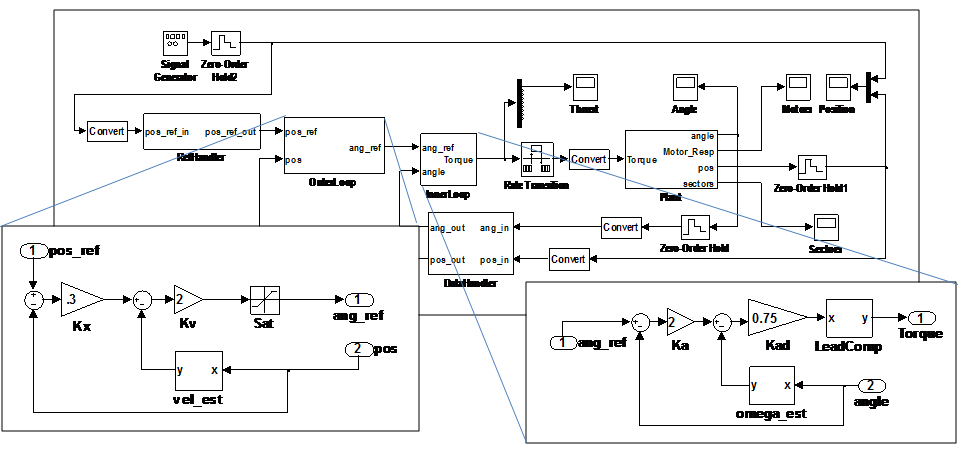
\includegraphics[width=\columnwidth]{figures/quadrotor_mdl.png}
    \caption{Simulink model of a simplified version of 
the quadrotor architecture.}
    \label{fig:qr_mdl}
\end{figure*}

\begin{figure}[thb]
\centering
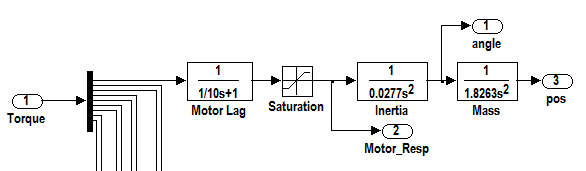
\includegraphics[width=0.8\columnwidth]{figures/quadrotor_plant.png}
    \caption{Simplified quadrotor plant dynamics.  The signal lines leading off the picture are signal taps used for online stability analysis.}
    \label{fig:qr_plant}
\end{figure}

Our second evaluation phase controls a continuous-time system whose model represents a simplified version of the quadrotor UAV.   This model still follows the  
basic component architecture for the control design (see Fig. \ref{fig:quadrotor}), but excludes the nonlinear rotational 
dynamics of the full quadrotor while retaining
the difficult coupled stability characteristics. Fig. \ref{fig:qr_plant} 
shows a Simulink model containing the simplified dynamics. The 
example model controls a stack of four integrators (and motor lag) 
using two nested PD control loops, as shown in the Simulink diagram of Fig. \ref{fig:qr_mdl}.  The Plant block contains the integrator models representing the vehicle dynamics. The two control loops (\emph{InnerLoop} and \emph{OuterLoop},
as shown in Fig. \ref{fig:qr_mdl}) are deployed to the Robostix and Gumstix
processors, respectively.  We refer to this example as the Quad Integrator model.  All of the controller components run at a frequency of 50Hz.  


Our controller evaluation method is based on sector theory, proposed originally by Zames\cite{control:sectors1} to analyze nonlinear elements in a control design.  Sectors provide two real-valued parameters which represent bounds on the possible input/output behaviors of a control loop.  Kottenstette presented a sector analysis block for validating a control design in Simulink\cite{quad:passcontrol}.  We propose to use the same structure to verify the deployed quadrotor control software online.  This method is described more fully in Porter et al\cite{pass:validation}.  A few concepts make this approach appealing for our case:

\begin{enumerate}
 \item For a given component, the sector measures behavior simultaneously over multiple inputs and outputs, so only one sector analyzer is required per control loop.
 \item Our passive abstraction of the system design (described below) allowed us to use a sector analyzer for each control loop to quickly isolate problem components in the deployed design.
\end{enumerate}

Passive control requires that controllers use energy received from inputs or stored previously, introducing no new energy into the environment\cite{pass:delasen}. If the plant dynamics were passive, we would have considerable freedom in setting gains and choosing control structures.  The zero-order hold outputs can introduce small amounts of new energy to the environment during rapid velocity changes, so each of the control loops must mitigate small amounts of ``active'' behavior.  The sector bound $a$ quantifies the energy-generating behavior of each control loop. In our quadrotor system, we expect the bound $a$ to be small and negative and choose the gains appropriately.  The result from Kottenstette indicates that the condition $k < -1/a$ is sufficient to ensure stability in these situations (where $k$ is the configured gain of the control loop)\cite{quad:passcontrol}.

\begin{figure*}[htb]
\centering
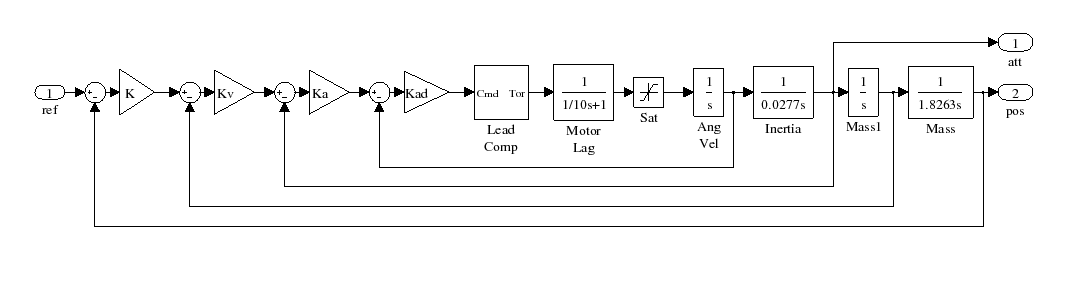
\includegraphics[width=\columnwidth]{figures/quadrotor_loops}
    \caption{Conceptual nested loop structure of the controller.}
    \label{fig:quadrotor_loops}
\end{figure*}

This particular design must be evaluated from the innermost loop to the outermost loop in order to make sense of the gain constraints. Fig. \ref{fig:quadrotor_loops} shows the nested loop structure of the design.  The actual design and implementation are complicated by the physical architecture of the digital realization: 

\begin{enumerate}
 \item Sensors acquire digital attitude and position information only, so velocities must be estimated.
 \item The controller components are deployed to different processors in the digital implementation, as described previously. Components on the two processors exchange data messages using a time-triggered protocol.
 \item Motor thrust commands are issued periodically using a zero-order hold.  As discussed previously the hold introduces additional energy back into the environment, violating the passivity condition.
\end{enumerate}

The sector blocks are attached around each controller, so input and output ports are oriented from the point of view of the control element.  The output of the controller (input to the rest of the system) is connected to the sector analyzer input port.  The signal controlled by the controller (before the error term is formed) is part of the input to the controller, but from our point of view it is the output of the system, so it connects to the sector
analyzer output port.  Fig. \ref{fig:sectorconn} displays the connection of the sector search block around the position control gain for our example. $K_x$ is the proportional gain for the outer loop PD controller, and $K_v$ is the derivative gain.  

\begin{figure}[htb]
\centering
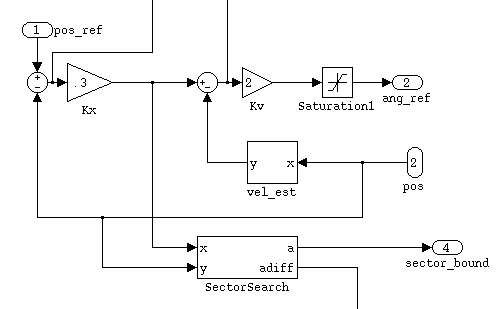
\includegraphics[width=0.75\columnwidth]{figures/sectorconn}
    \caption{Sector analysis block (\emph{SectorSearch}) connection around the position controller.}
    \label{fig:sectorconn}
\end{figure}


%TODO: Combine these plots side by side.

\begin{figure}[htb]
\centering
\subfloat[Simulink simulation.]{
\label{fig:sectors1} 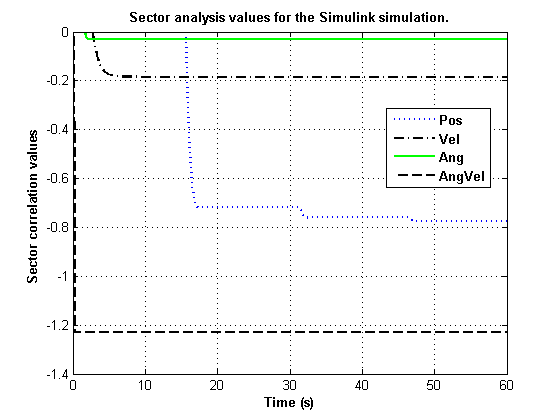
\includegraphics[width=0.48\columnwidth]{figures/simsectors}
}
%\end{figure}
%\begin{figure}[htb]
%\centering
\subfloat[Execution on hardware (including schedule effects).]{
\label{fig:sectors2} 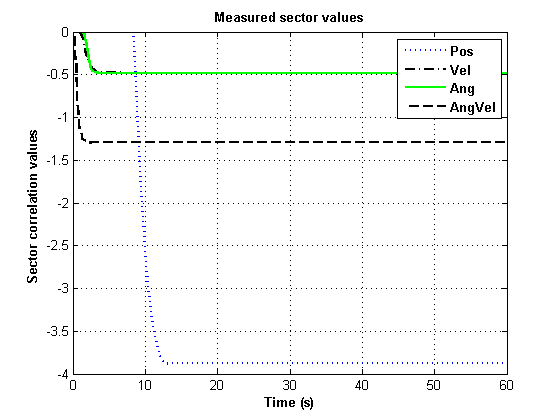
\includegraphics[width=0.48\columnwidth]{figures/meassectors}
}
\caption{Sector value evolution over time for the quad integrator.}
\label{fig:sectors}
\end{figure}

\begin{table*}[htb]
\centering

\begin{tabular}[width=0.95\columnwidth]{ | l | l | l | l | l | l | l | }

\hline
\textbf{Signal} & \textbf{Original} & \textbf{Simulated} & \textbf{Measured} & \textbf{Delta} & \textbf{New} & \textbf{New} \\
                & \textbf{Bound}    & \textbf{Sector}    & \textbf{Sector}  &                & \textbf{Bound} & \textbf{Sector} \\
\hline \hline
Angular Velocity & -1.333 & -1.2292 & -1.2963 & -0.0671 & -2.667 & -1.4568 \\
\hline
Angle & -0.5 & -0.0295 & -0.4831 & -0.4536 & -1.0 & -0.0068 \\
\hline
Velocity & -0.5 & -0.1856 & -0.4830 & -0.2974 & -1.0 &  -0.9324 \\
\hline
Position & -3.333 & -.7757 & -3.8811 & -3.1054 & -6.667 & -1.6081 \\
\hline
\end{tabular}
\caption{Sector value comparisons for simulation and execution on the actual platform.}
\label{tab:sectors}
\end{table*}

For this test we selected a square wave reference input near the highest frequency admissible by the controller.  Platform effects caused a significant deviation from our ideal sector estimates and bounds, as illustrated by the sector bound changes in Table \ref{tab:sectors}.  Fig. \ref{fig:sectors} illustrates the evolution of the collected sector data over time. For each digital control signal the table records the following (by column):
\begin{enumerate}
 \item Original Bound: the sector bound based on the original gain value ($-\frac{1}{k}$).
 \item Simulated Sector: the sector value recorded in simulation.
 \item Measured Sector: the initial sector value measured on the platform.
 \item Delta: the sector difference between the measured and simulated values.
 \item New Bound: the sector bound based on the newly adjusted gains.
 \item New Sector: the sector value measured on the platform with the new gains.
\end{enumerate}

Although the initial platform gains satisfied the sector stability conditions analytically and in simulation (comparing the Bound column to the Simulated column in the table), the overall system response when deployed to the target platform resulted in significant position overshoot.  The 
measured sector value for position measured the farthest from the predicted value, and exceeded the gain bound for stability ($-1/k$), though no evidence of instability was visible in the plot of the output trajectory.  As all of the gains moved right up to the edge of their bounds when deployed, we reduced all of the gains by $\frac{1}{2}$. Note that changing the gains changes the acceptable sector bound as well as the actual sector bounds themselves (as shown in Table \ref{tab:sectors}).  After adjusting the gains all of the sector values fell within the bounds.

On closer inspection we discovered that the most significant platform effect was a non-ideal position gain condition for signals with frequencies too close to the sampling rate.  Fig. \ref{fig:mags} shows a comparison of the ideal frequency response of the outer loop controller block with an empirically measured frequency response for the same controller
block deployed on the target hardware. Note the spike at the right-hand side of the plot in Fig. \ref{fig:mags}(b).  This is a nonlinear gain anomaly due to the effects of the saturation block, and which appears only for signals with frequencies right near the Nyquist sampling rate. The remedy was to add a simple input filter to cut off frequencies too close to the sampling rate. This effectively slows down the possible commands that can be issued to the system. The sector analysis blocks helped identify the position control component as the element whose behavior was farthest from predicted when 
deployed to the platform.   Adding a rate limiter block to the reference input resolved the problem.  Note that the full quadrotor model already included a 
similar (but more complex) rate limiter.

\begin{figure}[htb]
\centering
\subfloat[Analytically predicted response.]{
\label{fig:mags1} 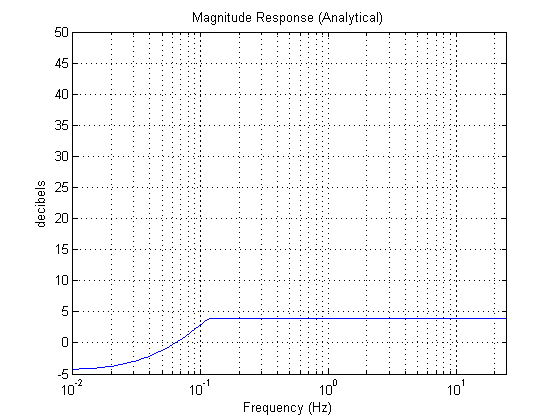
\includegraphics[width=0.48\columnwidth]{figures/magresp_analytical}
}
%\end{figure}
%\begin{figure}[htb]
%\centering
\subfloat[Measured response.]{
\label{fig:mags2} 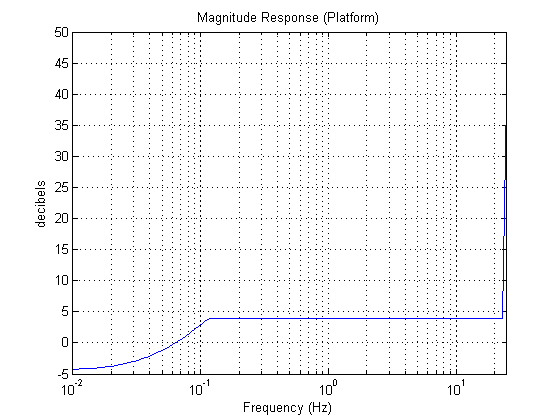
\includegraphics[width=0.48\columnwidth]{figures/magresp_platform}
}
\caption{Magnitude frequency responses for the quad integrator.}
\label{fig:mags}
\end{figure}

The Quad Integrator model simulation exposed a few interesting and
unanticipated defects in our design, beyond the gain anomaly detected by the sector analysis.  The most significant problem was the asynchronous arrival of the input sensor data.  Since the input data transfers were not synchronized with the controller schedule, we had to add a double-buffer to the UART data handler in order to eliminate data corruption.

\subsection{Quadrotor Model}

The final development phase integrated the full dynamics of the quadrotor,
comprised of the full data paths and nonlinear functions of the controllers.
Figs. \ref{fig:real_qr_mdl} - \ref{fig:real_qr_inner_loop} show details from the full Simulink model for the quadrotor.   
In the top-level design model (Fig. \ref{fig:real_qr_mdl}), the \emph{robo\_stix} block (Fig. \ref{fig:real_qr_robostix}) contains the functional specifications for the \emph{DataHandler} (\emph{sensor\_convert} block) and the \emph{InnerLoop} (\emph{inner\_loop} block, also Fig. \ref{fig:real_qr_inner_loop}) software components.  Likewise the \emph{gum\_stix} block and the \emph{ref\_data} block specify functions for the \emph{OuterLoop} and \emph{RefHandler} software components. 

\begin{figure}[thb]
\centering
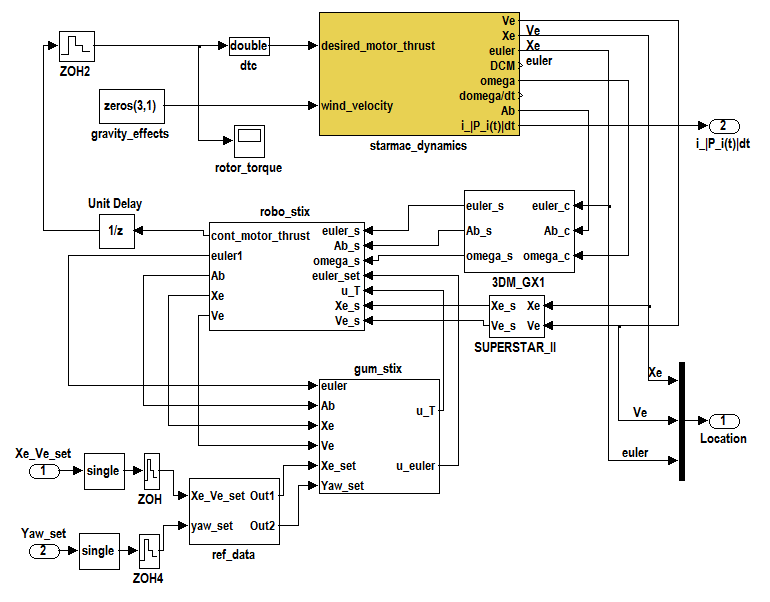
\includegraphics[width=0.8\columnwidth]{figures/real_quadrotor_mdl.png}
    \caption{Simulink model of the Starmac quadrotor helicopter.}
    \label{fig:real_qr_mdl}
\end{figure}

\begin{figure}[thb]
\centering
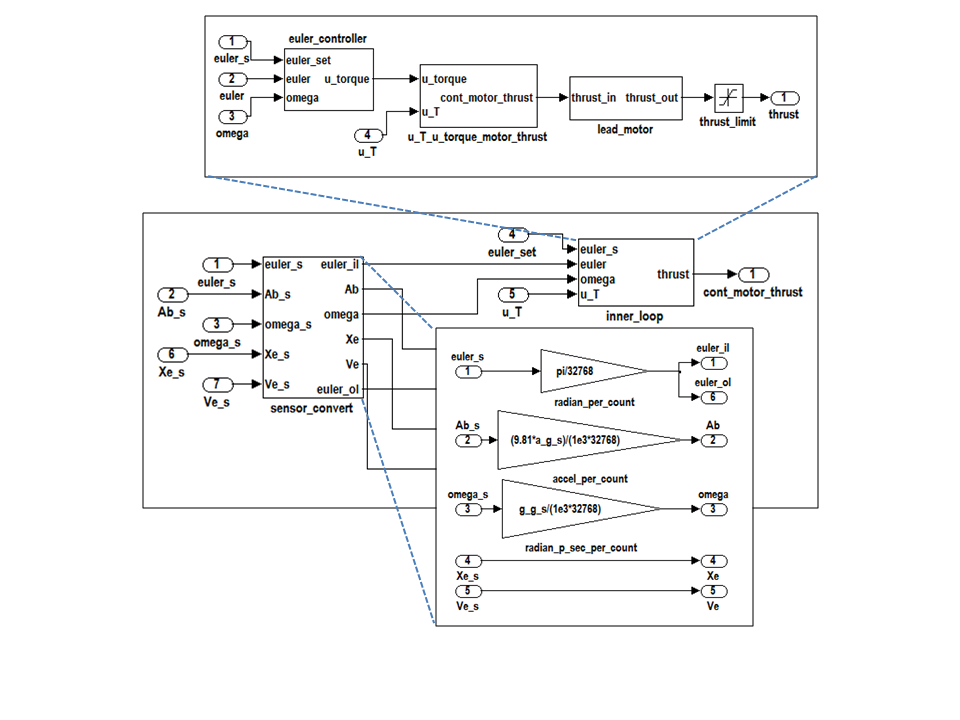
\includegraphics[width=0.8\columnwidth]{figures/real_quadrotor_rs_parts.png}
    \caption{Detail of the Robostix block.}
    \label{fig:real_qr_robostix}
\end{figure}

\begin{figure}[thb]
\centering
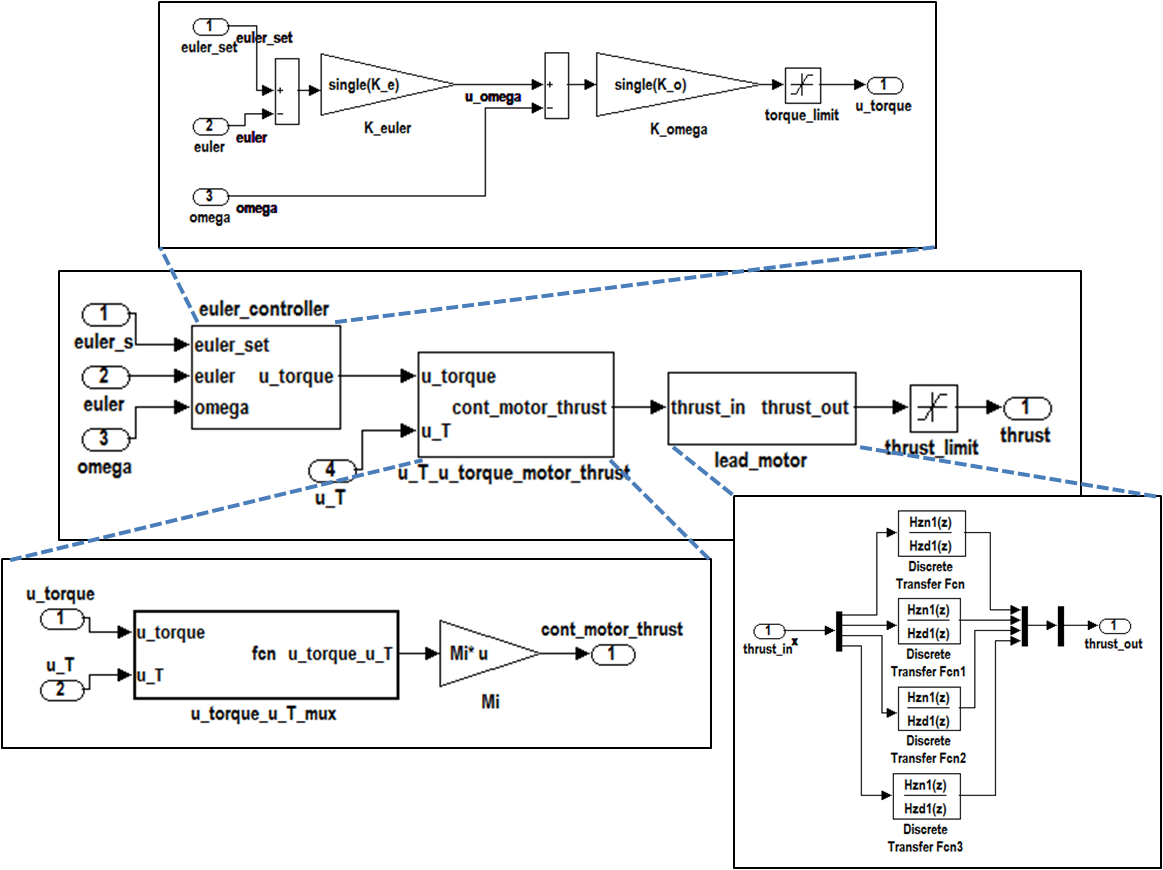
\includegraphics[width=0.9\columnwidth]{figures/real_quadrotor_inner_loop_parts.png}
    \caption{Detail of the inner loop block.}
    \label{fig:real_qr_inner_loop}
\end{figure}

We used the LogicPort probe to assess the correctness of the schedule.  
The configured schedule (Fig. \ref{fig:sched_schedviz}) correlates with the
schedule points measured by the LogicPort analyzer for the tasks and messages on the Robostix board (Fig. \ref{fig:sched_nodelays}).  Our experimental configuration did not provide a similar means for accurate measurement of the timing on the Gumstix board, though we can observe that message transfers start and end as predicted when task interference is absent.  Task interference was only observed
for misconfigured schedules, or when other non-controller Gumstix 
processes created heavy loads, delaying the controller.  Both schedule-based
and load-based interference were eliminated for nominal operation.
Fig. \ref{fig:qr_tracking} illustrates tracking behavior for the xPC-simulated Quadrotor, where the real-time controller implementation runs on the actual controller hardware.  The dashed curves represent the commanded $x$, $y$, and $z$ 
positions as shown, and the solid lines show the actual trajectory achieved by
the HIL simulated helicopter using the deployed controller code.

\begin{figure}[thb]
\centering
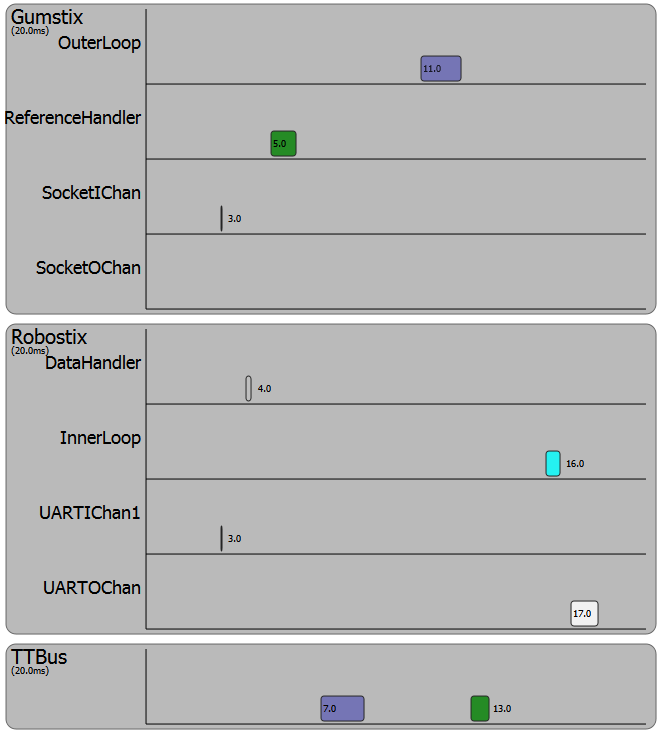
\includegraphics[width=0.8\columnwidth]{figures/qr_demo_schedviz.png}
    \caption{Schedule configuration for the quadrotor.}
    \label{fig:sched_schedviz}
\end{figure}

\begin{figure}[thb]
\centering
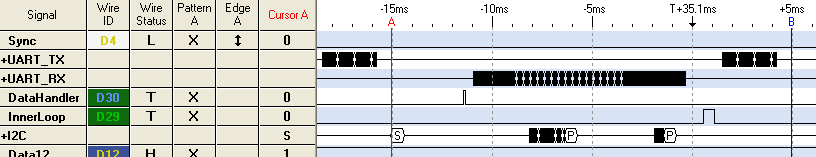
\includegraphics[width=\columnwidth]{figures/schedule_nodelays.png}
    \caption{Timing diagram for the Robostix AVR running the inner loop controller.}
    \label{fig:sched_nodelays}
\end{figure}

\begin{figure}[thb]
\centering
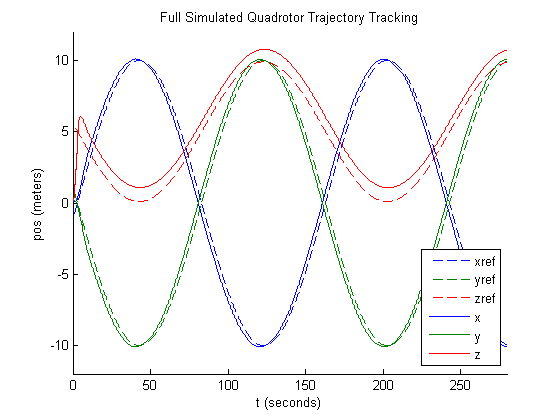
\includegraphics[width=\columnwidth]{figures/qr_tracking.png}
    \caption{Trajectory tracking for the quadrotor implementation.}
    \label{fig:qr_tracking}
\end{figure}

Our first move to the full quadrotor model uncovered numerical problems with some of the emulated floating-point functions provided by the gcc ARM cross-compiler.  This forced us to implement our own versions of the single-precision absolute value, signum, and minimum functions for the \emph{OuterLoop} component.  This problem was new to this phase of the evaluation because the rate limiter was not present in the Quad Integrator model.

\section{Lessons and Future Work}

%TODO: Talk about the moving parts in the quadrotor evaluation.  Include a diagram if possible.  

Probably the greatest difficulty in our work has been dealing with the large number of moving parts involved in the development of the modeling language and tools, the modeling and implementation of design examples, and the configuration of the development tools and execution environment for the target platform.  Our MIC-based solution only covered a part of the entire problem.   We only lightly addressed target system configuration, automated updates of the ESMoL model to track changes in the Simulink design, and runtime assessment (of both the simulator for plant dynamics and the target platform with the deployed code).  We developed a technique for runtime assessment of controller stability as covered in Porter et al\cite{pass:validation} (described partially in the Quad Integrator evaluation section), but it was difficult to automate due to the limited number of free data paths available for debugging in our chosen target system.   The integration of third party libraries in the development of our tools, and variations in platform module behavior were not directly addressed by our techniques, though they consumed 
significant development and testing time.

The next frontier in ESMoL development should be control loop modeling and analysis.  Control design formalisms abound, each with its own particular features and capabilities.  Passivity and the more general sector analysis formalisms are good examples of compositional frameworks which could be encoded in modeling tools\cite{ncs:mic} and which could support incremental development.

